\documentclass[12pt, pdf, hyperref={unicode},handout]{beamer}


\mode<presentation>
{
  \usetheme{Madrid}       % or try default, Darmstadt, Warsaw, ... Madrid
  \usecolortheme{orchid} % or try albatross, beaver, crane, ...default
  \usefonttheme{serif}    % or try default, structurebold, ... serif
  \usefonttheme{professionalfonts}
  \setbeamertemplate{navigation symbols}{}
   \setbeamertemplate{caption}[numbered]
} 
\usepackage{setspace}
\usepackage[english,russian]{babel}
\usepackage[utf8x]{inputenc}
\usepackage{hyperref}
\graphicspath{{images/}}
\definecolor{links}{HTML}{2A1B81}
\hypersetup{colorlinks,linkcolor=,urlcolor=links}
\colorlet{beamer@blendedblue}{green!40!black}
\usepackage{algorithmicx}
\usepackage{algpseudocode}

\usepackage{listings}



\setbeamertemplate{caption}[numbered]

\usepackage{ragged2e}
\renewcommand{\raggedright}{\leftskip=0pt \rightskip=0pt plus 0cm}

\usepackage{concmath}


\usepackage[orientation=landscape,size=A4,scale=4]{beamerposter}

\title[Искусственный интеллект]{Введение в предметную область ИИ}
\author[Артамонов Ю.Н.]{\small{\textit{Артамонов Юрий Николаевич \\  <<Экономика городского хозяйства и жилищного права>>}}}
\date[]{}
\institute[МГУУ]{\textbf{\textit{Государственное автономное образовательное учреждение высшего образования \\ <<Московский городской университет управления Правительства Москвы имени Ю.М. Лужкова>>}}}
\titlegraphic{
\includegraphics[width=4cm]{mguu}}


\begin{document}

\begin{frame}
  \titlepage
\end{frame}

% These three lines create an automatically generated table of contents.
\begin{frame}{Содержание}
  \tableofcontents
\end{frame}

\section{Основоположники направления ИИ}
\begin{frame}{\Large{Основоположники направления ИИ}}
\begin{block}
  
  \small{
\begin{center}
\begin{tabular}{ p{0.2\textwidth} p{0.25\textwidth} p{0.23\textwidth} p{0.23\textwidth}}
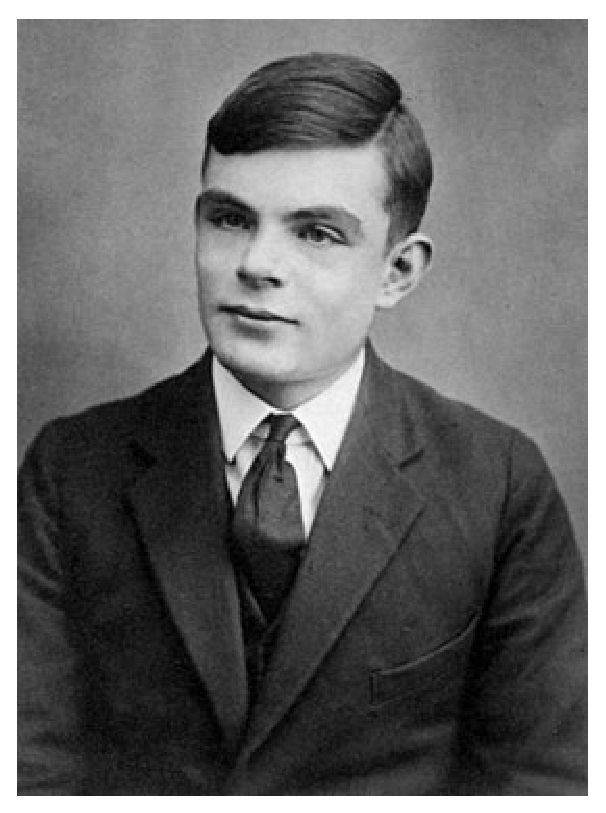
\includegraphics [scale=0.5]{ris2.eps}&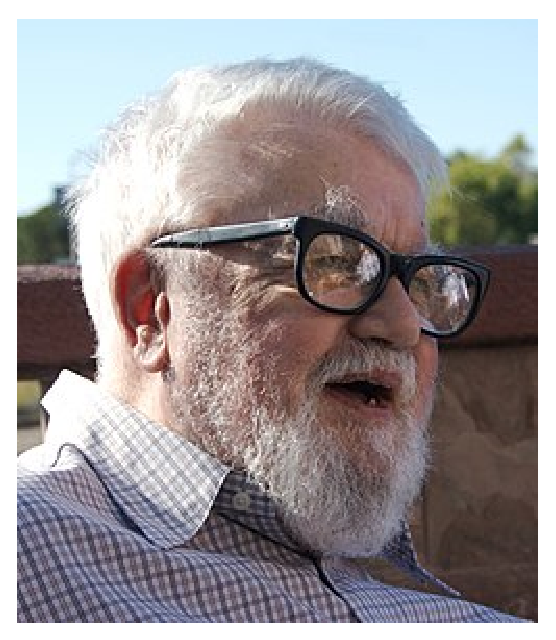
\includegraphics [scale=0.5]{ris1.eps}&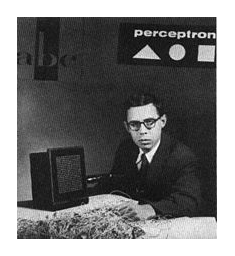
\includegraphics [scale=1.35]{ris3.eps}&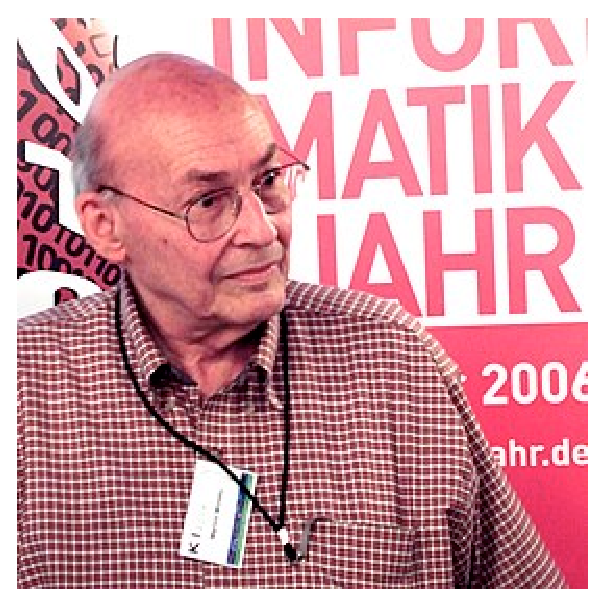
\includegraphics [scale=0.5]{ris4.eps}\\
\textbf{Алан Тьюринг} &  \textbf{Джон Маккарти} & \textbf{Фрэнк Розенблатт}& \textbf{Марвин Мински} \\  
1950 год:  & 1956 год: & 1958—1960:& 1967 год:\\
 \footnotesize{ИИ будет создан, когда человек общаясь с машиной, не сможет этого распознать.}  &\footnotesize{Проблема состоит в том, что пока мы не можем в целом определить, какие вычислительные процедуры мы хотим называть интеллектуальными. Поэтому под интеллектом  понимается только вычислительная составляющая способности достигать целей в мире.}  &  \footnotesize{Нельзя сказать, что мы точно воспроизводим работу человеческого мозга, - но пока перцептрон ближе всего к истине.}&\footnotesize{В течение поколения проблема создания ИИ будет практически решена. ... Через три-восемь лет у нас появится машина с интеллектом среднего человека.}
\end{tabular}
\end{center}
 
  }
  \end{block}

\end{frame}
\section{Перцептрон}
\begin{frame}{\Large{Перцептрон}}
\begin{block}
  
  \small{ 
    \begin{figure}[htb] 
      \centering
      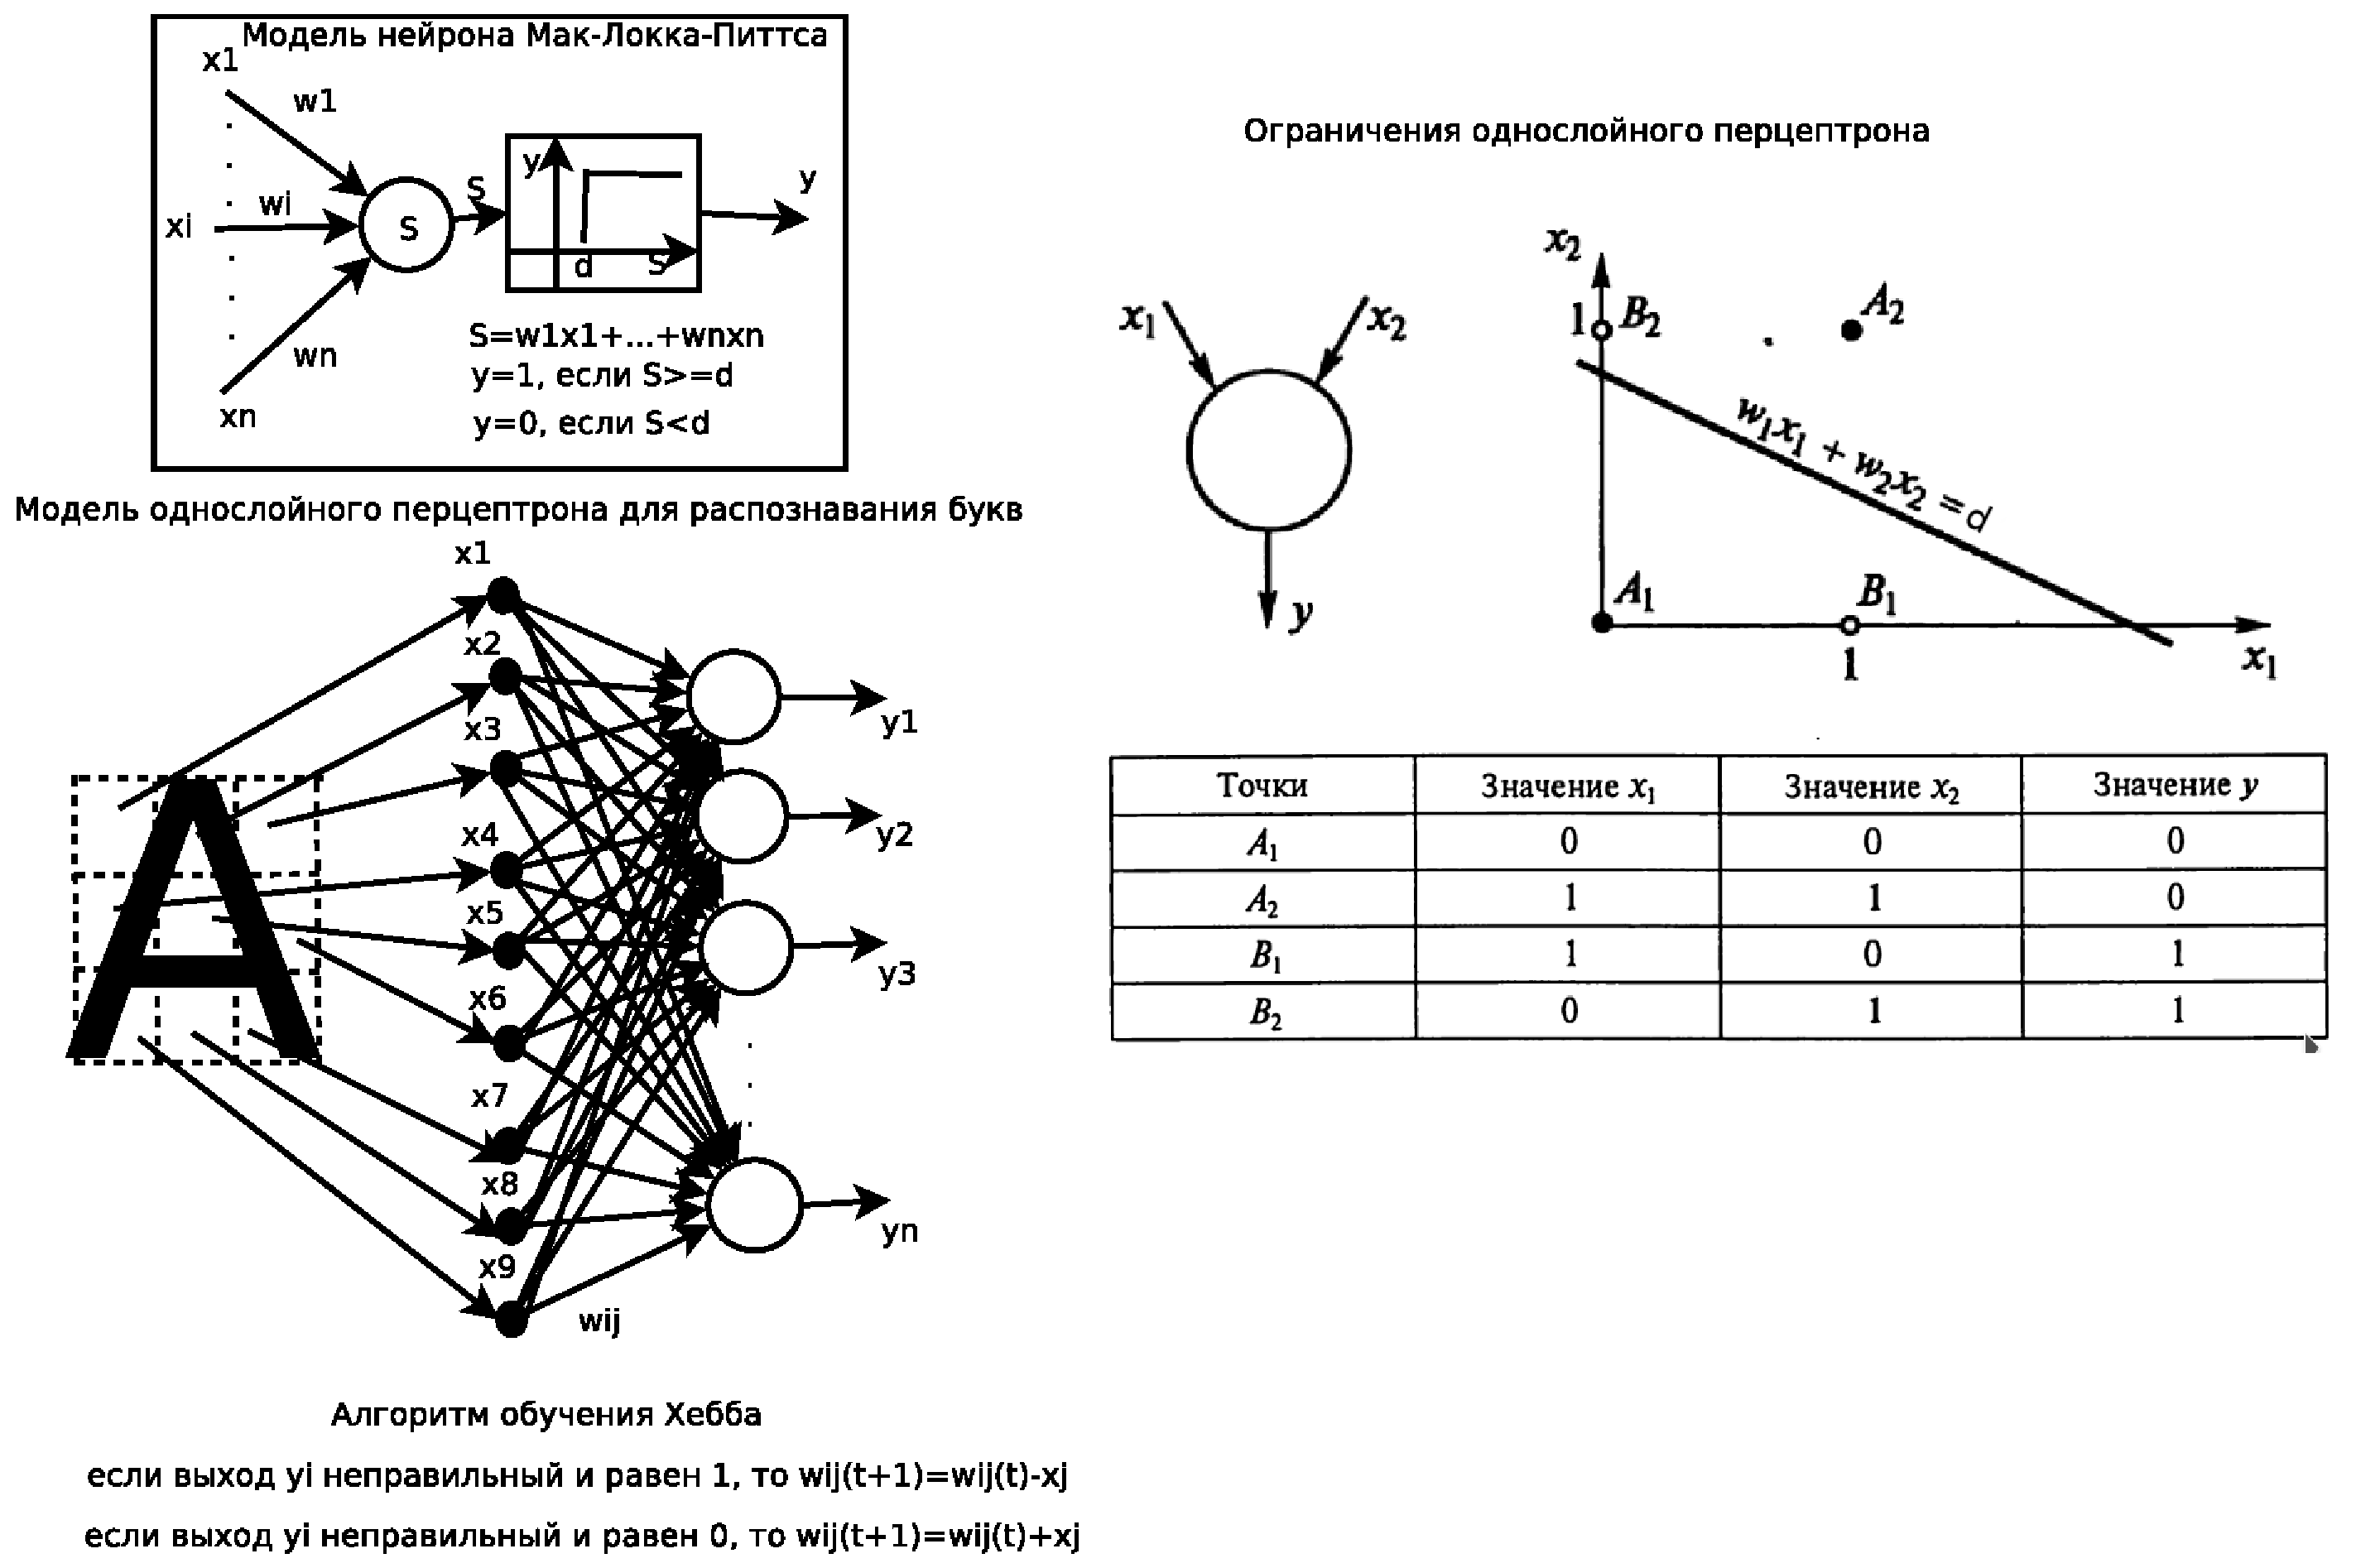
\includegraphics [scale=0.5]{ris5.eps}
    \end{figure} 
  }
  \end{block}

\end{frame}

\section{Функциональное, логическое программирование}
\begin{frame}{\Large{Рекурсия}}
\begin{block}{Идея рекурсии}
  
  \small{ 
    Пусть требуется реализовать вычисление $$sum(n)=1+2+3+\ldots +n$$
\begin{center}
  \begin{tabular}{ p{0.5\textwidth} p{0.5\textwidth}}
    Реализация без рекурсии&Реализация с рекурсией\\
  \begin{algorithmic}[1]
\Function{sum}{$n$}
\State $result\gets 0, i\gets 1$
\While{$i\leq n$}
\State $result\gets result+i$
\State $i\gets i+1$
\EndWhile
\State \textbf{return} $result$
\EndFunction
\end{algorithmic} &
 \begin{algorithmic}[1]
\Function{sum}{$n$}
\If {$n=0$}
\State \textbf{return} $0$
\Else
\State \textbf{return} $sum(n-1)+n$
\EndIf
\EndFunction
\end{algorithmic}
    \\
\end{tabular}
\end{center}
 
  }
  \end{block}

\end{frame}

\begin{frame}{\Large{Рекурсия}}
\begin{block}{Идея рекурсии - попытка понять}
  
  \small{ 
$$sum(n)=sum(n-1)+n$$
$$sum(n-1)=sum(n-2)+(n-1)$$
$$\ldots$$
$$sum(1)=sum(0)+1$$
$$sum(0)=0$$
\begin{center}
  \begin{tabular}{ p{0.25\textwidth} p{0.7\textwidth}}
    \textbf{Задача о ханойской башне}& \textbf{Рекурсивный алгоритм}\\
  \begin{figure}[htb] 
    \centering
    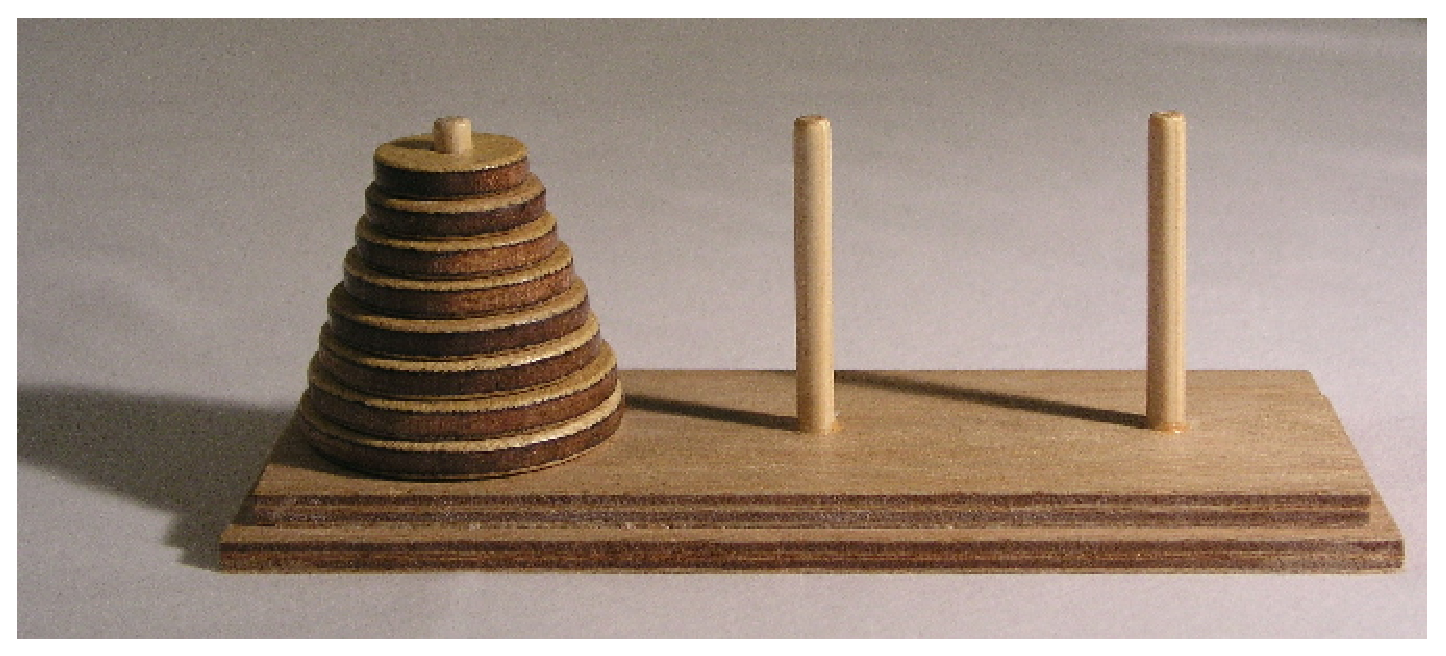
\includegraphics [scale=0.3] {hanoy.eps}
  \end{figure} &
  Предположим, что мы уже научились перекладывать n-1 колец, тогда алгоритм перекладывания n колец такой:
    \begin{itemize}
    \item{перекладываем на средний колышек n-1 колец }
    \item{перекладываем на крайний правый колышек самое большое кольцо}
    \item{перекладываем на крайний правый колышек n-1 колец }
    \item{Последовательно уменьшая n мы приходим к одному кольцу, алгоритм перекладывания которого очевиден.}
    \end{itemize}\\
    \end{tabular}
\end{center}
  }
  \end{block}

\end{frame}

\begin{frame}{\Large{Функциональное программирование - символьные вычисления}}
\begin{block}{}
  
  \small{ 
    \begin{figure}[htb] 
      \centering
      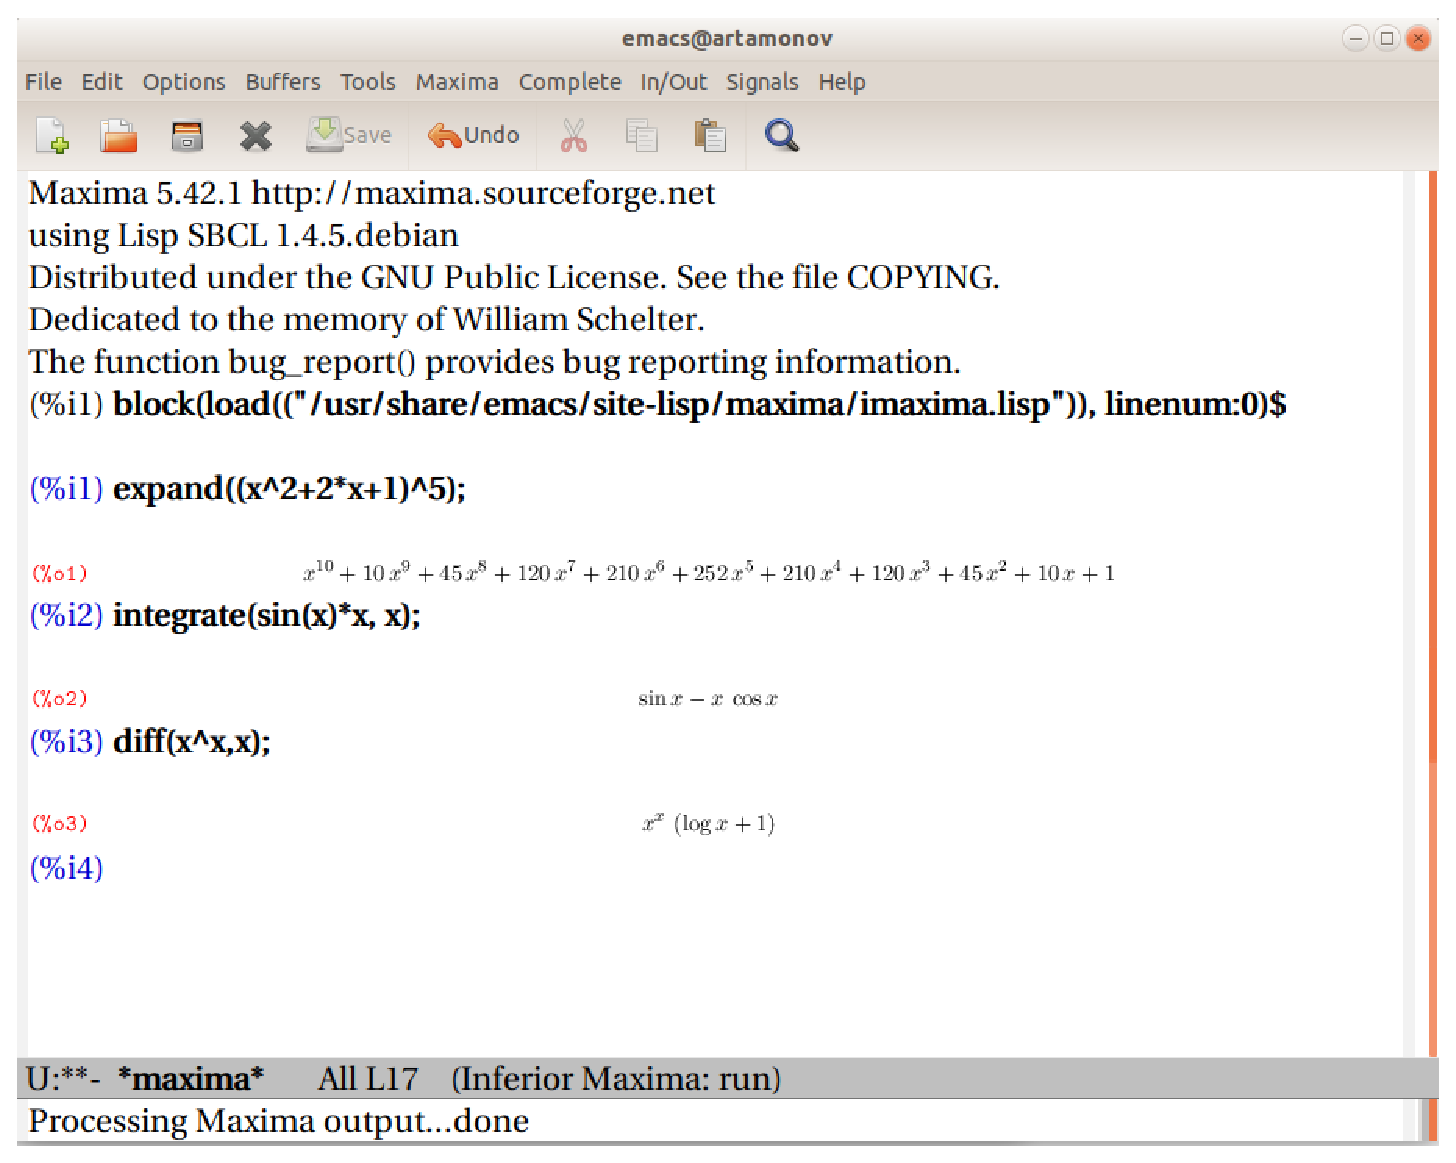
\includegraphics [scale=0.8]{ris51.eps}
    \end{figure}

    \href{https://www.wolframalpha.com}{Mathematica — система компьютерной алгебры:} https://www.wolframalpha.com
  }
  \end{block}

\end{frame}

\begin{frame}{\Large{Логическое программирование - Пролог}}
\begin{block}
  
  \small{ 
    \begin{figure}[htb] 
      \centering
      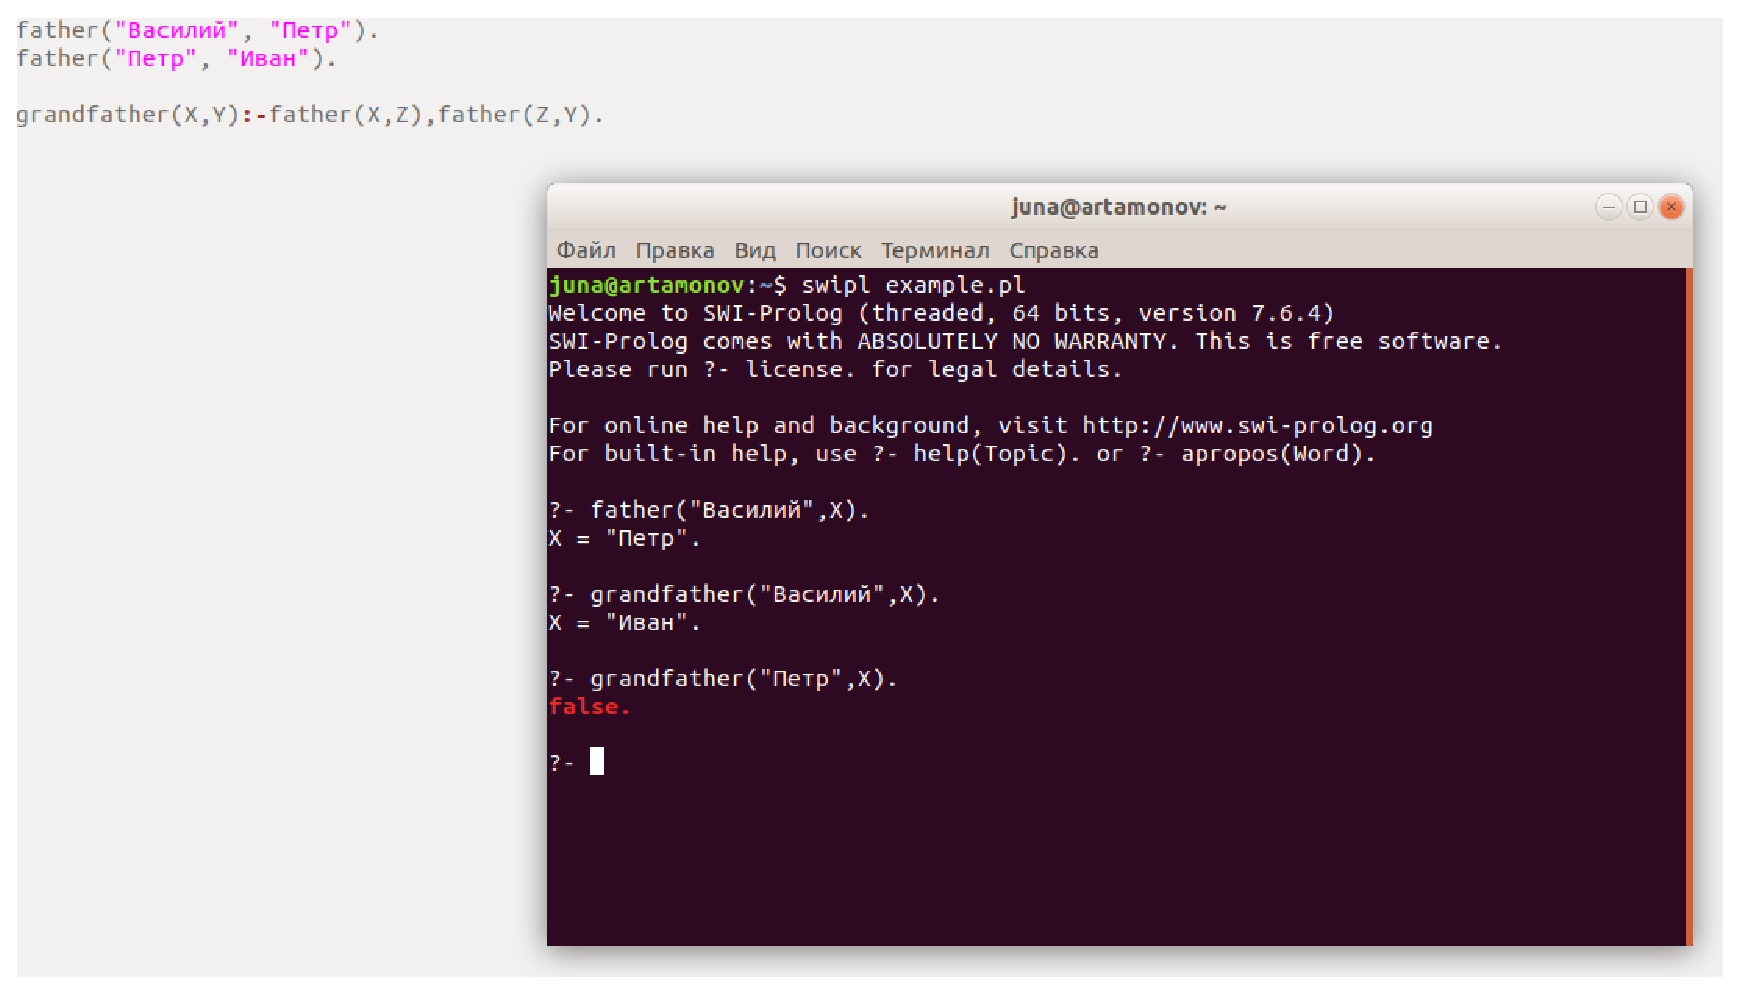
\includegraphics [scale=0.9]{ris6.eps}
    \end{figure} 
  }
  \end{block}

\end{frame}

\begin{frame}{\Large{Логическое программирование - Пролог}}
\begin{block}{Задача про козу, волка и капусту}
  
  \small{
    Старик должен переправить на другой берег реки волка, козу и капусту. При этом существует два ограничения:
    \begin{itemize}
  \item{Его лодка такова, что за один раз может вместе с ним перевезти только кого-то одного: либо волка, либо козу, либо капусту.}
  \item{Звери мирно ведут себя только в присутствии старика. Стоит только ему отлучиться, как волк тут же съест козу или коза съест капусту.}
    
   \href{https://rextester.com/l/prolog_online_compiler}{Пролог онлайн}: https://rextester.com/l/prolog\_online\_compiler
  \end{itemize}
    \begin{figure}[htb] 
      \centering
      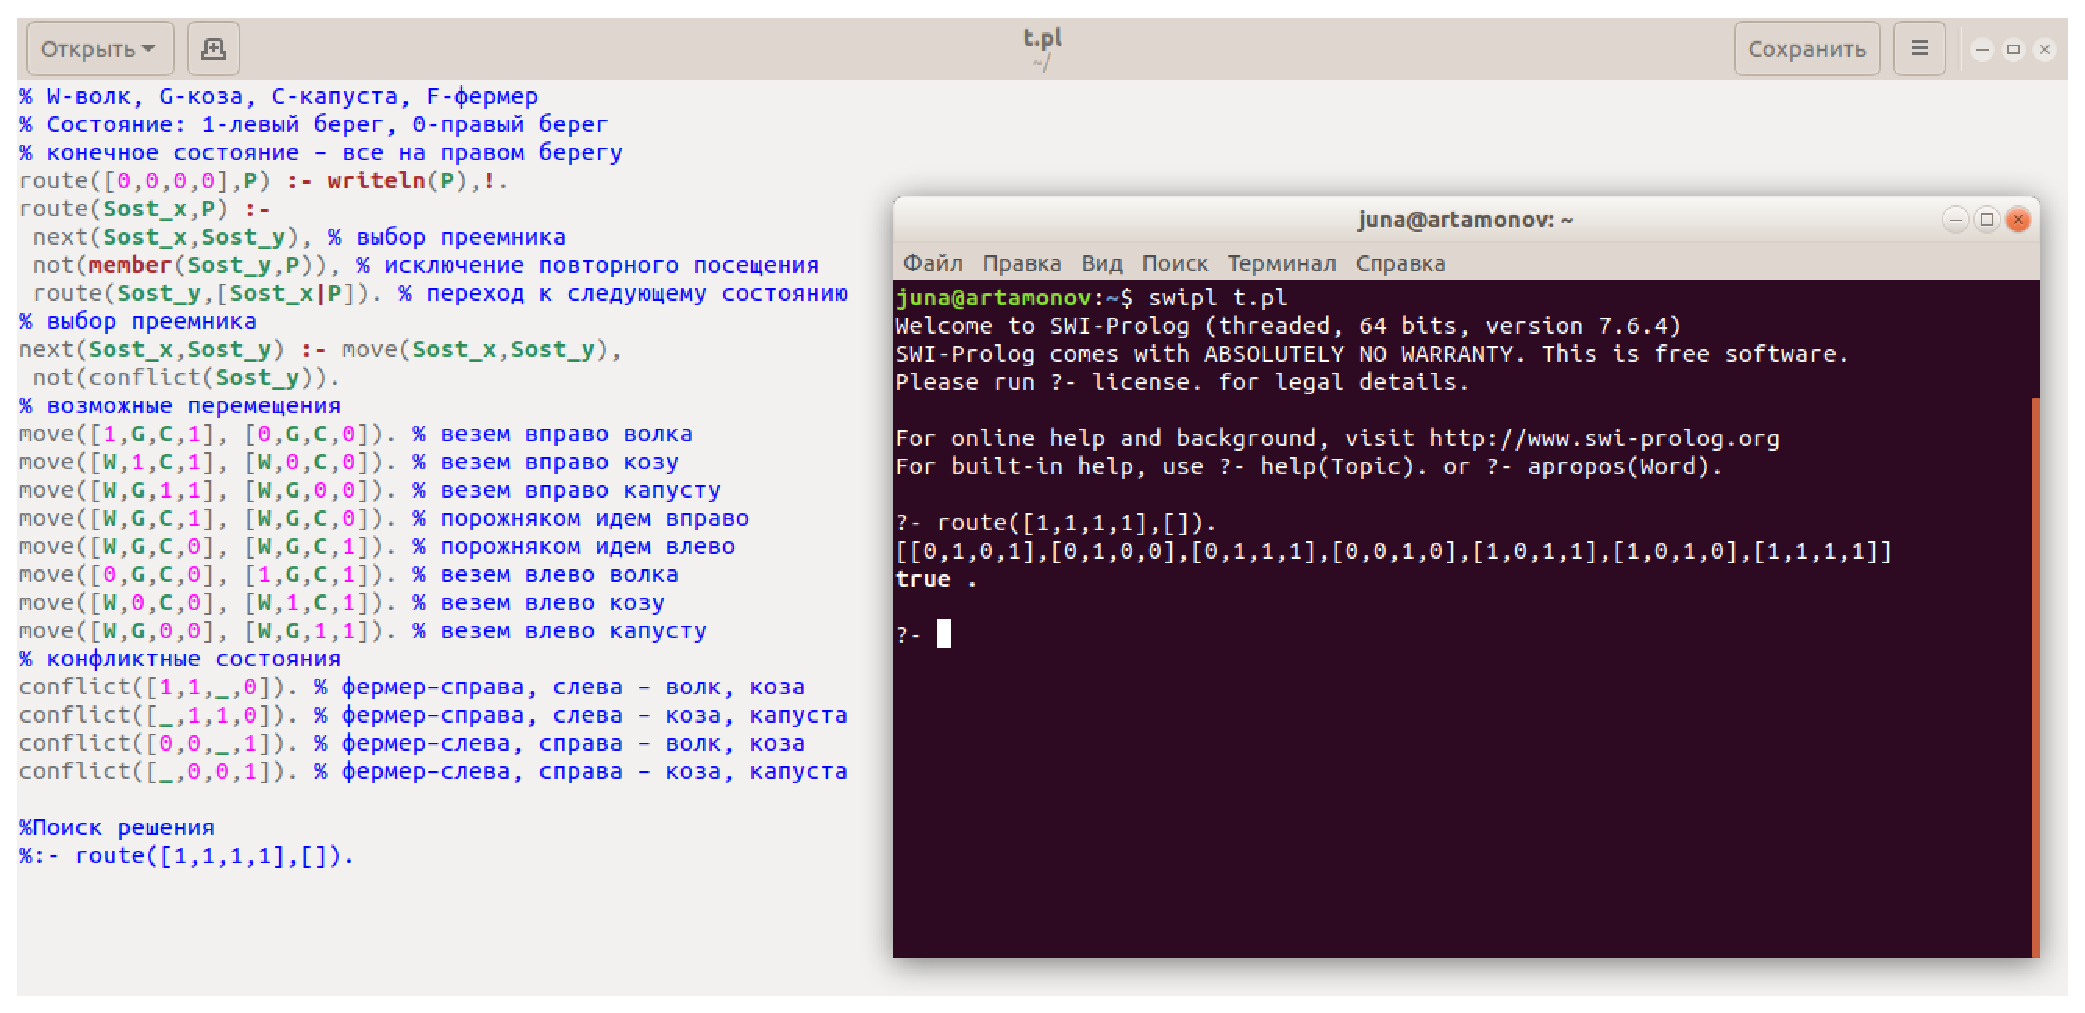
\includegraphics [scale=0.6]{ris7.eps}
    \end{figure} 
  }
  
  \end{block}

\end{frame}

\begin{frame}{\Large{Слабый и сильный ИИ}}
  
    \begin{figure}[htb] 
      \centering
      \includegraphics [scale=3.3]{SSAI.png}
    \end{figure} 


\end{frame}

\begin{frame}{\Large{Слабый ИИ - экспертные системы 1980 г.г.}}
\begin{block}
  
В начале 80-х годов получили широкое распространение экспертные системы — программы, имитирующие знания и умения человека. Для создания таких программ проводился подробный опрос экспертов с целью выяснить, каким именно образом они решают задачи, например, по каким правилам психолог отвечает пациенту или врач определяет диагноз. Полученные правила затем реализовывались в виде компьютерной программы. Однако и эти системы быстро достигли своего потолка, положив начало второй «зиме искусственного интеллекта». Тем не менее, экспертные системы по-прежнему используются в некоторых областях, особенно в тех, в которых особое внимание уделяется надежности, например в медицине.
  
  \end{block}

\end{frame}

\begin{frame}{\Large{Слабый ИИ }}
\begin{block}

  \small{
  \textbf{1990 г. - Deep Blue}
  
В конце 90-х годов XX века и начале XXI века драйверами развития искусственного интеллекта стали увеличивающиеся вычислительные мощности, активное применение математических методов, а также упор на решение конкретных задач. Искусственный интеллект начал использоваться в различных областях: в логистике, экономике, медицине. Одним из известных прорывов стала разработка суперкомпьютера Deep Blue, обыгравшего в 1997 году действующего чемпиона мира по шахматам Гарри Каспарова.

\textbf{2000 г. - Данные}

В начале XXI века одним из основных драйверов разработки алгоритмов искусственного интеллекта стали данные, а акценты в сфере искусственного интеллекта сместились в сторону таких областей, как машинное обучение, анализ больших данных и др. В отличие от экспертных систем, формализующих человеческий опыт в виде программы, машинное обучение извлекает знания из большой базы данных, благодаря чему получается более точный алгоритм, корректно работающий в более широком круге случаев.
 } 
  \end{block}

\end{frame}

\begin{frame}{\Large{Слабый ИИ }}
\begin{block}

  \small{
  \textbf{2010-е: Watson и DeepMind}
  
В 2011 году компания IBM представила систему Watson, способную находить ответы на вопросы, заданные на естественном языке. Для демонстрации навыков система «сыграла» в игру «Jeopardy!» (американский аналог русскоязычной «Своей игры») и обыграла обоих соперников. В основе Watson — алгоритмы информационного поиска, обработки естественного языка, машинного обучения и построения логических цепочек.

В 2015 году британская компания DeepMind (один из крупнейших сегодняшних лидеров в области искусственного интеллекта) представила AlphaGo — систему, обыгравшую чемпиона мира по игре в Го, Ли Седоля. Го намного сложнее шахмат из-за большего количества возможных позиций, что создает сложности в применении алгоритмов поиска ходов, активно используемых в DeepBlue. Основу AlphaGo составляют алгоритмы машинного обучения: программа обучалась на данных 160 тысяч партий профессионалов.

 } 
  \end{block}

\end{frame}

\begin{frame}{\Large{Слабый ИИ?}}
\begin{block}

  \small{
  \textbf{2020: GPT-3, AlphaFold}
  
В 2020 году американская компания OpenAI представила систему GPT-3, способную генерировать англоязычные тексты, неотличимые от написанных человеком, с сохранением темы по всему объему текста, грамматической корректностью и т. д.

В том же 2020 году компания DeepMind представила AlphaFold, решающую задачу прогноза третичной структуры белков, которая являлась одной из сложнейших и важнейших задач в современной биологии и решение которой не могли найти около 50 лет.

 } 
  \end{block}

\end{frame}

\section{Основные термины и определения}
\begin{frame}{\Large{Основные определения и термины}}
\begin{block}

  \small{
 \textbf{Искусственный интеллект} - это комплекс технологических решений, позволяющий имитировать
когнитивные функции человека и получать при выполнении
конкретных задач результаты, сопоставимые, как минимум,
с результатами интеллектуальной деятельности человека

Искусственный интеллект включает в себя множество областей

\begin{figure}[htb] 
      \centering
      \includegraphics [scale=2.7]{Obj.png}
    \end{figure}

 } 
  \end{block}

\end{frame}

\begin{frame}{\Large{Основные определения и термины}}
\begin{block}

  \small{
 
 \textbf{Машинное обучение}

Класс методов искусственного интеллекта, характерной чертой которых является не прямое решение задачи, а обучение в процессе применения решений множества сходных задач.

\textbf{Глубинное обучение}

Иногда называют «глубокое обучение» (от англ. Deep learning). Подобласть машинного обучения, где в качестве алгоритмов используются нейронные сети.

\textbf{Data Science}

Это концепция объединения статистики, анализа данных, машинного обучения и связанных с ними методов для понимания и анализа реальных явлений.

\textbf{Data Mining}

Широкое понятие, означающее извлечение знаний из данных.

\textbf{Большие данные}

Это набор подходов и методов, разработанных для анализа данных огромных размеров.
 } 
  \end{block}

\end{frame}

\section{Задачи машинного обучения}

\begin{frame}{\Large{Задачи машинного обучения}}
\begin{block}


    \begin{itemize}
    \item{Классификация}
    \item{Регрессия}
    \item{Кластеризация}
    \item{Понижение размерности}
    \item{Важность признаков}
    \item{Ассоциации, рекомендации}
    \end{itemize}

  
  \end{block}

\end{frame}

\begin{frame}{\Large{Демонстрация метода кластеризации k-means}}
  
\begin{block}

\begin{figure}[htb] 
      \centering
      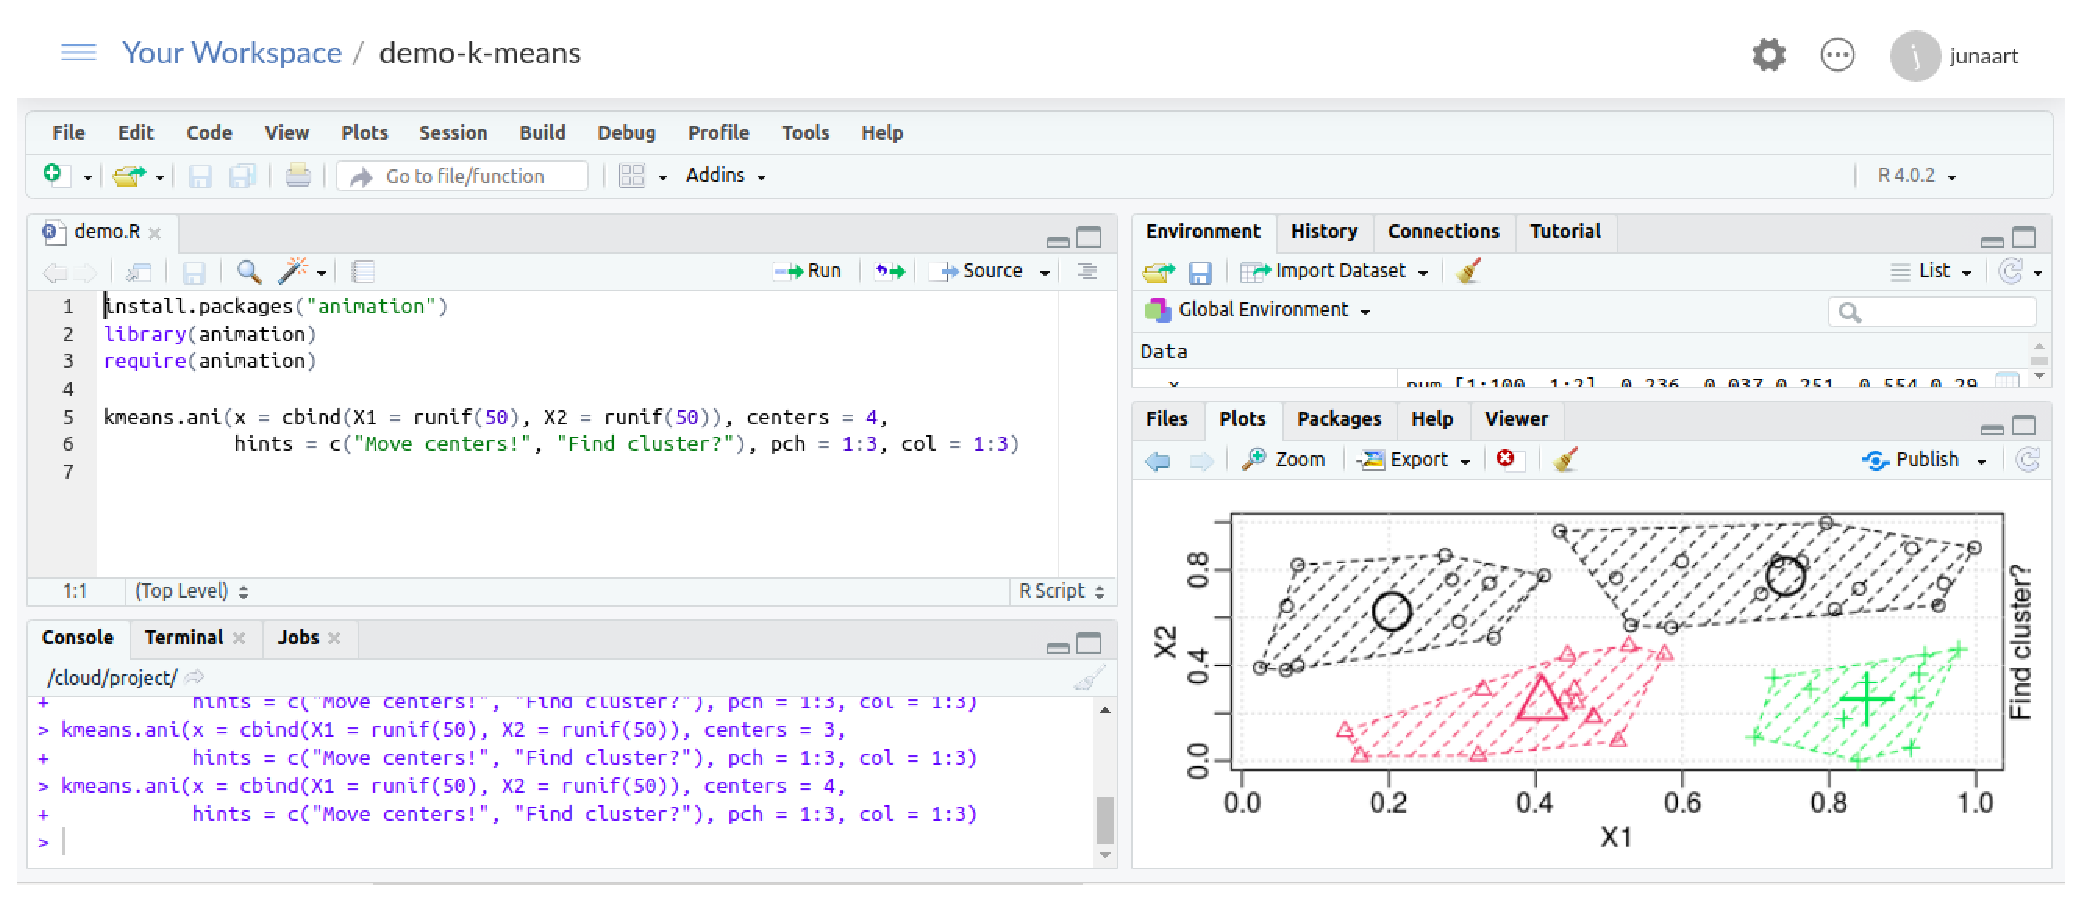
\includegraphics [scale=0.8]{ris8.eps}
\end{figure}

 \url{https://posit.cloud/content/1732717}

\end{block}

\end{frame}

\begin{frame}[fragile]{\Large{Пример использования нейронных сетей: решение задачи <<исключающее или>> }}
\begin{block}{}

  \begin{lstlisting}[language=R]
install.packages("neuralnet")
library(neuralnet)
x1<-c(0,0,1,1)
x2<-c(0,1,0,1)
y<-c(0,1,1,0)

d<-data.frame(x1,x2,y)
View(d)

nn=neuralnet(y~x1+x2,data=d, hidden=c(3,4,5))
plot(nn)
xx<-data.frame(x1,x2)
result<-predict(nn,xx)
View(data.frame(d,result))
  \end{lstlisting}

 \end{block}
\end{frame}

\begin{frame}{\Large{Пример использования нейронных сетей: решение задачи <<исключающее или>> }}
\begin{block}{}

  \begin{figure}[htb] 
      \centering
      \includegraphics [scale=2.5]{ris13.png}
    \end{figure}

    Работа с кодом доступна по ссылке:

    \url{https://posit.cloud/content/1713842}

 \end{block}
\end{frame}

\begin{frame}[fragile]{\Large{Пример использования нейронных сетей: решение задачи <<Классификация ирисов>>}}
\begin{block}{}

  \small{
  \begin{lstlisting}[language=R]
x<-c(1:150)
y<-sample(x,floor(150*0.8))
z<-setdiff(x,y)
D_teach<-iris[y,]
D_test<-iris[z,]
nn=neuralnet(class ~ sl + sw + pl + pw,data=
D_teach, hidden=c(3,4,5))
plot(nn)

g<-predict(nn,D_teach)
colnames(g)<-c("setosa","versicolor","virginica")
View(data.frame(D_teach$class,g))

g<-predict(nn,D_test)
colnames(g)<-c("setosa","versicolor","virginica")
View(data.frame(D_test$class,g))

\end{lstlisting}

}

 \end{block}
\end{frame}

\begin{frame}{\Large{Пример использования нейронных сетей: решение задачи <<Классификация ирисов>>}}
\begin{block}{}

  \begin{figure}[htb] 
      \centering
      \includegraphics [scale=2.5]{ris14.png}
    \end{figure}

    Работа с кодом доступна по ссылке:

    \url{https://posit.cloud/content/1713842}

 \end{block}
\end{frame}

\section{Современное состояние, тенденции, выводы}

\begin{frame}{\Large{Глубинное обучение: элементы теории нейронных сетей}}
\begin{block}{Различные варианты нейронных сетей}

  \begin{figure}[htb] 
      \centering
      \includegraphics [scale=0.55]{ris12.png}
    \end{figure}

 \end{block}
\end{frame}

\begin{frame}{\Large{Глубинное обучение: популярные архитектуры нейросетей}}
  \begin{block}{Анализ изображений - сверточные нейронные сети}

    \small{Первый сверточный слой применяется непосредственно к самому изображению, второй слой — к выходу первого сверточного слоя и т. д. Выход сверточного слоя формально тоже является изображением, но на глубоких слоях нейронной сети это «изображение» уже не будет интерпретироваться человеком. Между сверточными слоями, как и между полносвязными, вставляют слои нелинейности, а в конце сверточной архитектуры обычно вставляют один или несколько полносвязных слоев.}
    
  \begin{figure}[htb] 
      \centering
      \includegraphics [scale=3.5]{svert.png}
    \end{figure}

 \end{block}
\end{frame}

\begin{frame}{\Large{Глубинное обучение: популярные архитектуры нейросетей}}
  \begin{block}{Анализ изображений - сверточные нейронные сети}

    \small{В сверточных нейросетях при увеличении номера сверточного слоя повышается уровень абстракции. Первые слои распознают простые переливы яркости и отдельные цвета, слои чуть глубже распознают простые геометрические формы, еще более глубокие слои распознают части изображений, например глаза, губы и нос при анализе лиц, а самые глубокие слои отвечают за распознавание целых объектов.}
    
  \begin{figure}[htb] 
      \centering
      \includegraphics [scale=3.5]{svert2.png}
    \end{figure}

 \end{block}
\end{frame}

\begin{frame}{\Large{Глубинное обучение: популярные архитектуры нейросетей}}
  \begin{block}{Задачи анализа изображений}
    
  \begin{figure}[htb] 
      \centering
      \includegraphics [scale=3.5]{svert3.png}
    \end{figure}

 \end{block}
\end{frame}

\begin{frame}{\Large{Глубинное обучение: популярные архитектуры нейросетей}}
  \begin{block}{Задачи генерации изображений}

    \small{За последние несколько лет произошел прорыв в решении обратной задачи — генерации фотореалистичных изображений и видео. Как и в анализе изображений, в генерации изображений используются сверточные нейронные сети. На вход нейросети подаются характеристики изображения, которое нужно сгенерировать, а на выход нейросеть выдает новое изображение.}
  \begin{figure}[htb] 
      \centering
      \includegraphics [scale=3.5]{svert4.png}
    \end{figure}

 \end{block}
\end{frame}

\begin{frame}{\Large{Глубинное обучение: популярные архитектуры нейросетей}}
  \begin{block}{Задачи генерации изображений}

    \small{Перенос стиля работает так: на вход нейросети подаются два изображения — то, которое нужно перерисовать, и то, с которого нужно скопировать стиль, а на выход выдается стилизованное изображение.}
  \begin{figure}[htb] 
      \centering
      \includegraphics [scale=3.5]{svert5.png}
    \end{figure}
    \small{Смена времени дня на фотографиях}
  

 \end{block}
\end{frame}

\begin{frame}{\Large{Глубинное обучение: популярные архитектуры нейросетей}}
  \begin{block}{Задачи генерации изображений}

    \small{Чтобы генерировать фотореалистичные изображения, используют так называемые генеративно-состязательные сети (generative adversarial networks, GAN).

      GAN состоит из двух нейросетей: первая генерирует изображение, а вторая решает задачу классификации и учится определять, на входе настоящее оно или сгенерированное. Задача первой нейросети — "обмануть" вторую, и она "вынуждена" генерировать реалистичные кадры.}
\begin{figure}[htb] 
      \centering
      \includegraphics [scale=2]{svert6.png}
    \end{figure}
    \small{Лица знаменитостей, сгенерированных нейросетью}

 \end{block}
\end{frame}

\begin{frame}{\Large{Глубинное обучение: популярные архитектуры нейросетей}}
  \begin{block}{Kandinsky - новые возможности генерации изображений}

\begin{figure}[htb] 
      \centering
      \includegraphics [scale=2.9]{svert7.png}
    \end{figure}

 \end{block}
\end{frame}

\begin{frame}{\Large{Попробуйте сами!}}
  \begin{block}{Kandinsky 2.2 - телеграмм-бот}

\begin{figure}[htb] 
      \centering
      \includegraphics [scale=6]{svert8.png}
    \end{figure}

 \end{block}
\end{frame}

\begin{frame}{\Large{Глубинное обучение: популярные архитектуры нейросетей}}
  \begin{block}{Анализ текстов - рекуррентные нейронные сети, трансформеры}

 \small{
    Область обработки текстов по-английски называется \textbf{Natural Language processing (NLP)}.
    
    \textbf{Алгоритм обработки текстов}
    \begin{itemize}
      \item{\textbf{Предобработка текстов}. Перед тем, как обучать алгоритм на данных, их необходимо подготовить к обработке: очистить и собрать словарь, который нейросеть потом будет использовать для перевода текста на "машинный" язык. В результате предобработки каждый текст представляется в виде последовательности номеров слов в словаре. }
      \item{\textbf{Векторные представления слов(эмбединги)}. Для каждого слова в словаре слой извлекает набор чисел фиксированного размера, например 256 чисел — этот набор и называется векторным представлением, или эмбеддингом. У разных слов — разные векторные представления. При этом часто получается, что у слов, близких по смыслу, векторные представления похожи. Каждое число в эмбеддинге соответствует какому-то «смыслу».}
    \item{\textbf{Использование рекуррентного слоя или архитектуры трансформер}}
    \end{itemize}
}
    
 \end{block}
\end{frame}

\begin{frame}{\Large{Глубинное обучение: популярные архитектуры нейросетей}}
  \begin{block}{Рекуррентные нейронные сети}

 \small{
Основная идея рекуррентного слоя — повторение одной и той же процедуры обработки для каждого слова.

Внутри рекуррентный слой устроен как полносвязный слой: в качестве входных нейронов выступают эмбеддинг слова и предыдущее скрытое состояние, в качестве выходных нейронов — новое скрытое состояние. Самое первое скрытое состояние обычно делают состоящим из нулей. Рекуррентных слоев можно использовать несколько, один за другим. В результате получится рекуррентная нейронная сеть (Recurrent Neural Network, RNN).
}

\begin{figure}[htb] 
      \centering
      \includegraphics [scale=0.7]{rec.png}
    \end{figure}

    
 \end{block}
\end{frame}

\begin{frame}{\Large{Глубинное обучение: популярные архитектуры нейросетей}}
  \begin{block}{Трансформеры}

 \small{
Недостатки рекуррентных нейросетей, отсутствие связи между далекими словами и забывание слов, были исправлены в другой архитектуре, называемой Трансформер.

В Трансформере новое скрытое состояние для слова вычисляется на основе векторных представлений всех остальных слов.

В итоге каждое слово связано с каждым и проблем с учетом «длинных» зависимостей нет. Обычно Трансформер состоит из четырех или шести слоев, каждый из которых включает попарные связи.
}

\begin{figure}[htb] 
      \centering
      \includegraphics [scale=0.8]{trans.png}
    \end{figure}

    
 \end{block}
\end{frame}

\begin{frame}{\Large{Глубинное обучение: популярные архитектуры нейросетей}}
  \begin{block}{Задачи анализа текстов}

 \small{
   \begin{itemize}
   \item{\textbf{Задача классификации текстов.} Например, обнаружение спама, оскорбений и т.п.}
   \item{\textbf{Задача регрессии.}  Например, по тексту объявления о вакансии предсказывать заработную плату.}
   \item{\textbf{Задача тегирования} -  нужно выполнить отдельное предсказание для каждого слова в тексте. К этой группе относятся задача определения частей речи для каждого слова и задача определения синтаксических ролей в предложении — такие алгоритмы помогают, в частности, выполнять автокоррекцию текста.}
   \item{\textbf{Задача выделения именованных сущностей} -  найти в тексте города, компании, персоналии и другие объекты реального мира. }
     \item{\textbf{Задача генерации текста.} }
     \end{itemize}

     Сказать, что нейросети достигли полного понимания текстов, написанных людьми, и способны генерировать абсолютно качественные тексты самостоятельно, пока нельзя, однако существенный прорыв в области NLP уже произошел.
     
 }
 
 \end{block}
\end{frame}

\section{Генеративный искусственный интеллект}

\begin{frame}{\Large{Развитие моделей семейства GPT}}
\begin{block}{Прорывы и открытия в мире языковых моделей}

 \begin{figure}[htb] 
      \centering
      \includegraphics [scale=1]{pror.png}
    \end{figure}

 \end{block}
\end{frame}


\begin{frame}{\Large{Генеративный искусственный интеллект}}
\begin{block}{Общие сведения о чат боте}

  \small{
  ChatGPT — нейросеть для генерации текстового контента, и обучали ее на огромных массивах текста из Интернета. Хорошо понимает разные языки. Может просто общаться, помогать решать задачи, писать программы на языке программирования, генерировать изображения. Однако сеть неидеальна и правильность своих ответов она не гарантирует, но она умеет обучаться и корректировать свое поведение. Текущая доступная рабочая версия 3.5.

  В России прямой доступ к чат боту заблокирован, но имеется возможность доступа через телеграмм каналы.

  На текущий момент компания OpenAI анонсировала новую версию GPT-4. На их официальном сайте появилось следующее сообщение:

  GPT-4 — это большая мультимодальная модель (принимающая изображения и текст на входе и выводящая текст на выходе), которая, хотя и хуже, чем люди во многих реальных сценариях, демонстрирует производительность на уровне человека в различных профессиональных и академических тестах.
  }

 \end{block}
\end{frame}




\begin{frame}{\Large{Примеры использования ChartGPT}}
\begin{block}{Программируем...}

  \begin{figure}[htb] 
      \centering
      \includegraphics [scale=3]{ris17.png}
    \end{figure}

 \end{block}
\end{frame}

\begin{frame}{\Large{Примеры использования ChartGPT}}
\begin{block}{Решаем...}

  \begin{figure}[htb] 
      \centering
      \includegraphics [scale=3.5]{ris18.png}
    \end{figure}

 \end{block}
\end{frame}

\begin{frame}{\Large{Попробуйте сами!}}
  \begin{block}{ChatGPT4 - телеграмм-бот}

\begin{figure}[htb] 
      \centering
      \includegraphics [scale=2]{qrgpt.png}
    \end{figure}

 \end{block}
\end{frame}

\begin{frame}{\Large{Попробуйте сами!}}
  \begin{block}{Deepseek}

\begin{figure}[htb] 
      \centering
      \includegraphics [scale=8]{deepseek.png}
    \end{figure}

    \url{https://chat.deepseek.com/}

 \end{block}
\end{frame}

\begin{frame}{\Large{Генеративный искусственный интеллект}}
\begin{block}{Отличия ChartGPT-4}

  \small{

  А еще известно:
  \begin{itemize}
  \item{GPT-4 предусматривает несколько способов взаимодействия с человеком - не только с помощью ввода текста, но также при голосовом общении, отправкой изображения, звука или видео. }
\item{ИИ сможет как воспринимать информацию в виде файлов и видео, так и генерировать в таком же формате. То есть он сможет делать музыку, видео по текстовому сообщению. }
\item{Ответы ChatGPT при использовании модели GPT-4 будут ещё более человечными, то есть сильнее приближенными к речи, которую обычно используют люди, общаясь друг с другом. }
\item{GPT-4 будет поддерживать "буквально все языки".}
\item{GPT-4 будет в 537 раз способнее своего предшественника.}
\end{itemize}
}

 \end{block}
\end{frame}

\begin{frame}{\Large{Генеративный искусственный интеллект}}
  \begin{block}{}

  \begin{figure}[htb] 
      \centering
      \includegraphics [scale=1]{gpt4.png}
    \end{figure}

 \end{block}
\end{frame}



\begin{frame}{\Large{Все пытаются построить свой GPT}}
  \begin{block}

    
    
  \begin{figure}[htb] 
      \centering
      \includegraphics [scale=0.95]{change.png}
    \end{figure}

 \end{block}
\end{frame}

\begin{frame}{\Large{Сравнение языковых моделей}}
  \begin{block}{Сравнение по числу параметров, длина контекста, доступность в Open-Source}

    
    
  \begin{figure}[htb] 
      \centering
      \includegraphics [scale=1]{srav.png}
    \end{figure}

 \end{block}
\end{frame}

\begin{frame}{\Large{Текущие возможности}}
  \begin{block}

    
    
  \begin{figure}[htb] 
      \centering
      \includegraphics [scale=0.95]{AIpossible.png}
    \end{figure}

 \end{block}
\end{frame}

\begin{frame}{\Large{Индекс качества}}
  \begin{block}

    
    
  \begin{figure}[htb] 
      \centering
      \includegraphics [scale=3.5]{2025_1.png}
    \end{figure}

 \end{block}
\end{frame}

\begin{frame}{\Large{Понимание языка, рассуждения}}
  \begin{block}

    
    
  \begin{figure}[htb] 
      \centering
      \includegraphics [scale=3.5]{2025_2.png}
    \end{figure}

 \end{block}
\end{frame}

\begin{frame}{\Large{Научные рассуждения, знания}}
  \begin{block}

    
    
  \begin{figure}[htb] 
      \centering
      \includegraphics [scale=3.5]{2025_3.png}
    \end{figure}

 \end{block}
\end{frame}


\begin{frame}{\Large{Решение математических задач}}
  \begin{block}

    
    
  \begin{figure}[htb] 
      \centering
      \includegraphics [scale=3.5]{2025_4.png}
    \end{figure}

 \end{block}
\end{frame}

\begin{frame}{\Large{Генерация кода}}
  \begin{block}

    
    
  \begin{figure}[htb] 
      \centering
      \includegraphics [scale=3.5]{2025_5.png}
    \end{figure}

 \end{block}
\end{frame}

\begin{frame}{\Large{Стоимость обучения}}
  \begin{block}

    
    
  \begin{figure}[htb] 
      \centering
      \includegraphics [scale=3.5]{2025_6.png}
    \end{figure}

 \end{block}
\end{frame}

\begin{frame}{\Large{Будущее искусственного интеллекта}}
  \begin{block}{Настоящее - будущее}

    
    
  \begin{figure}[htb] 
      \centering
      \includegraphics [scale=1]{FutureAI.png}
    \end{figure}

 \end{block}
\end{frame}


\section{Основные тренды цифровой экономики}
\begin{frame}{\Large{Основные тренды мирового развития в области цифровой экономики}}
\begin{block}

 \large{
  \begin{itemize}
  \item{Большие данные.}
  \item{Нейротехнологии и искусственный интеллект.}
  \item{Интернет вещей.}
  \item{Системы распределенного реестра <<Блокчейн>>.}
  \item{Технологии виртуальной и дополненной реальности.}
    \item{Квантовые компьютеры.}
  \end{itemize}
}
 
  \end{block}

\end{frame}

\begin{frame}{\Large{Правовое регулирование цифровизации в России}}
\begin{block}{Основные инициативы национальной программы  \\ <<Цифровая экономика России>>}

  \Large{
 \begin{itemize}
  \item{Регулирование цифровой среды.}
  \item{Информационная инфраструктура.}
  \item{Кадры для цифровой экономики.}
  \item{Информационная безопасность.}
  \item{Цифровые технологии.}
  \item{Цифровое государственное управление.}
  \item{Искусственный интеллект.}
  \end{itemize}
  }

 \end{block}
\end{frame}

\section{Цифровые проекты и сервисы в городском хозяйстве Москвы}

\begin{frame}{\Large{Государственные программы города Москвы}}
\begin{block}

  \begin{figure}[htb] 
      \centering
      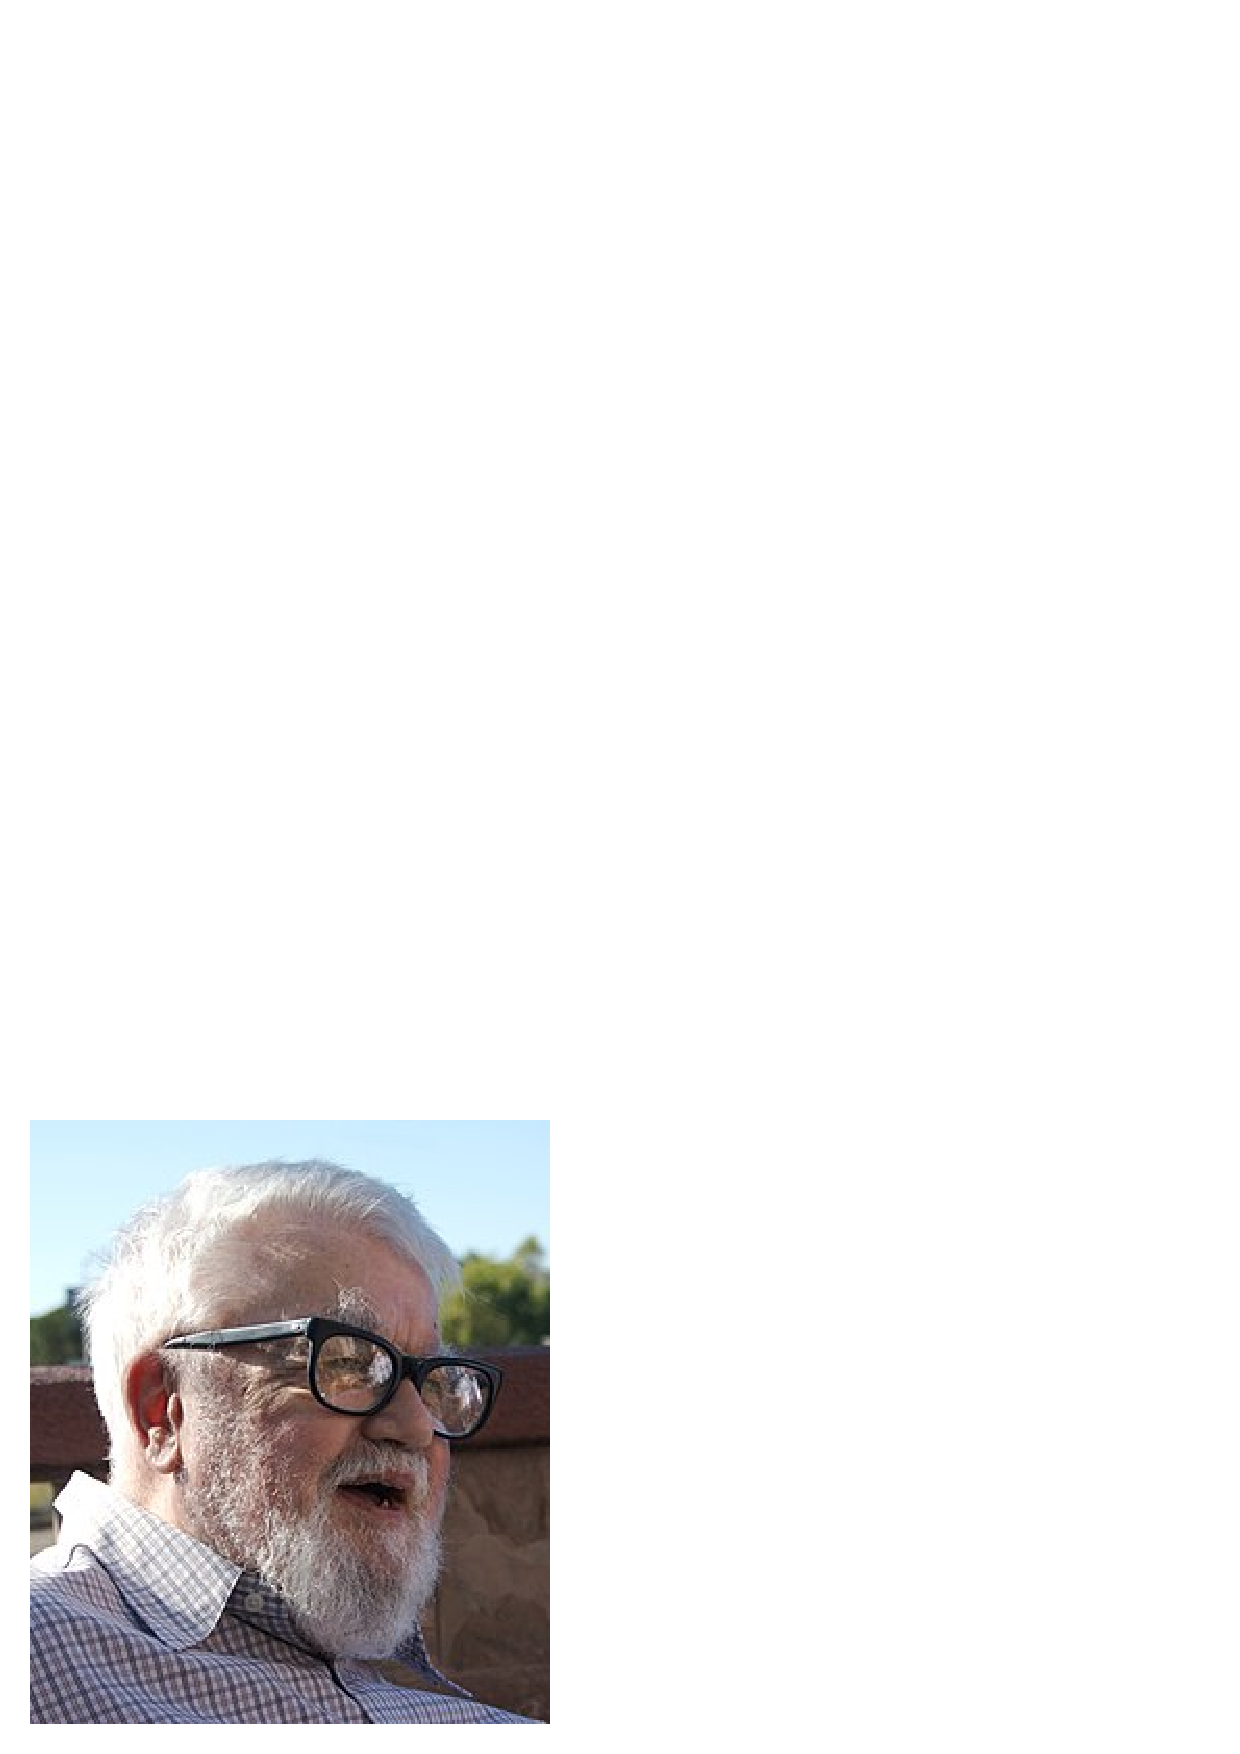
\includegraphics [scale=0.7]{ris1.png}
    \end{figure} 
  

  \small{Источник: https://budget.mos.ru/budget/gp}
  
 \end{block}
\end{frame}



\begin{frame}{\Large{Направления цифровизации в городе Москве}}
\begin{block}{Официальный портал Мэра и Правительства Москвы (mos.ru)}

  \begin{figure}[htb] 
      \centering
      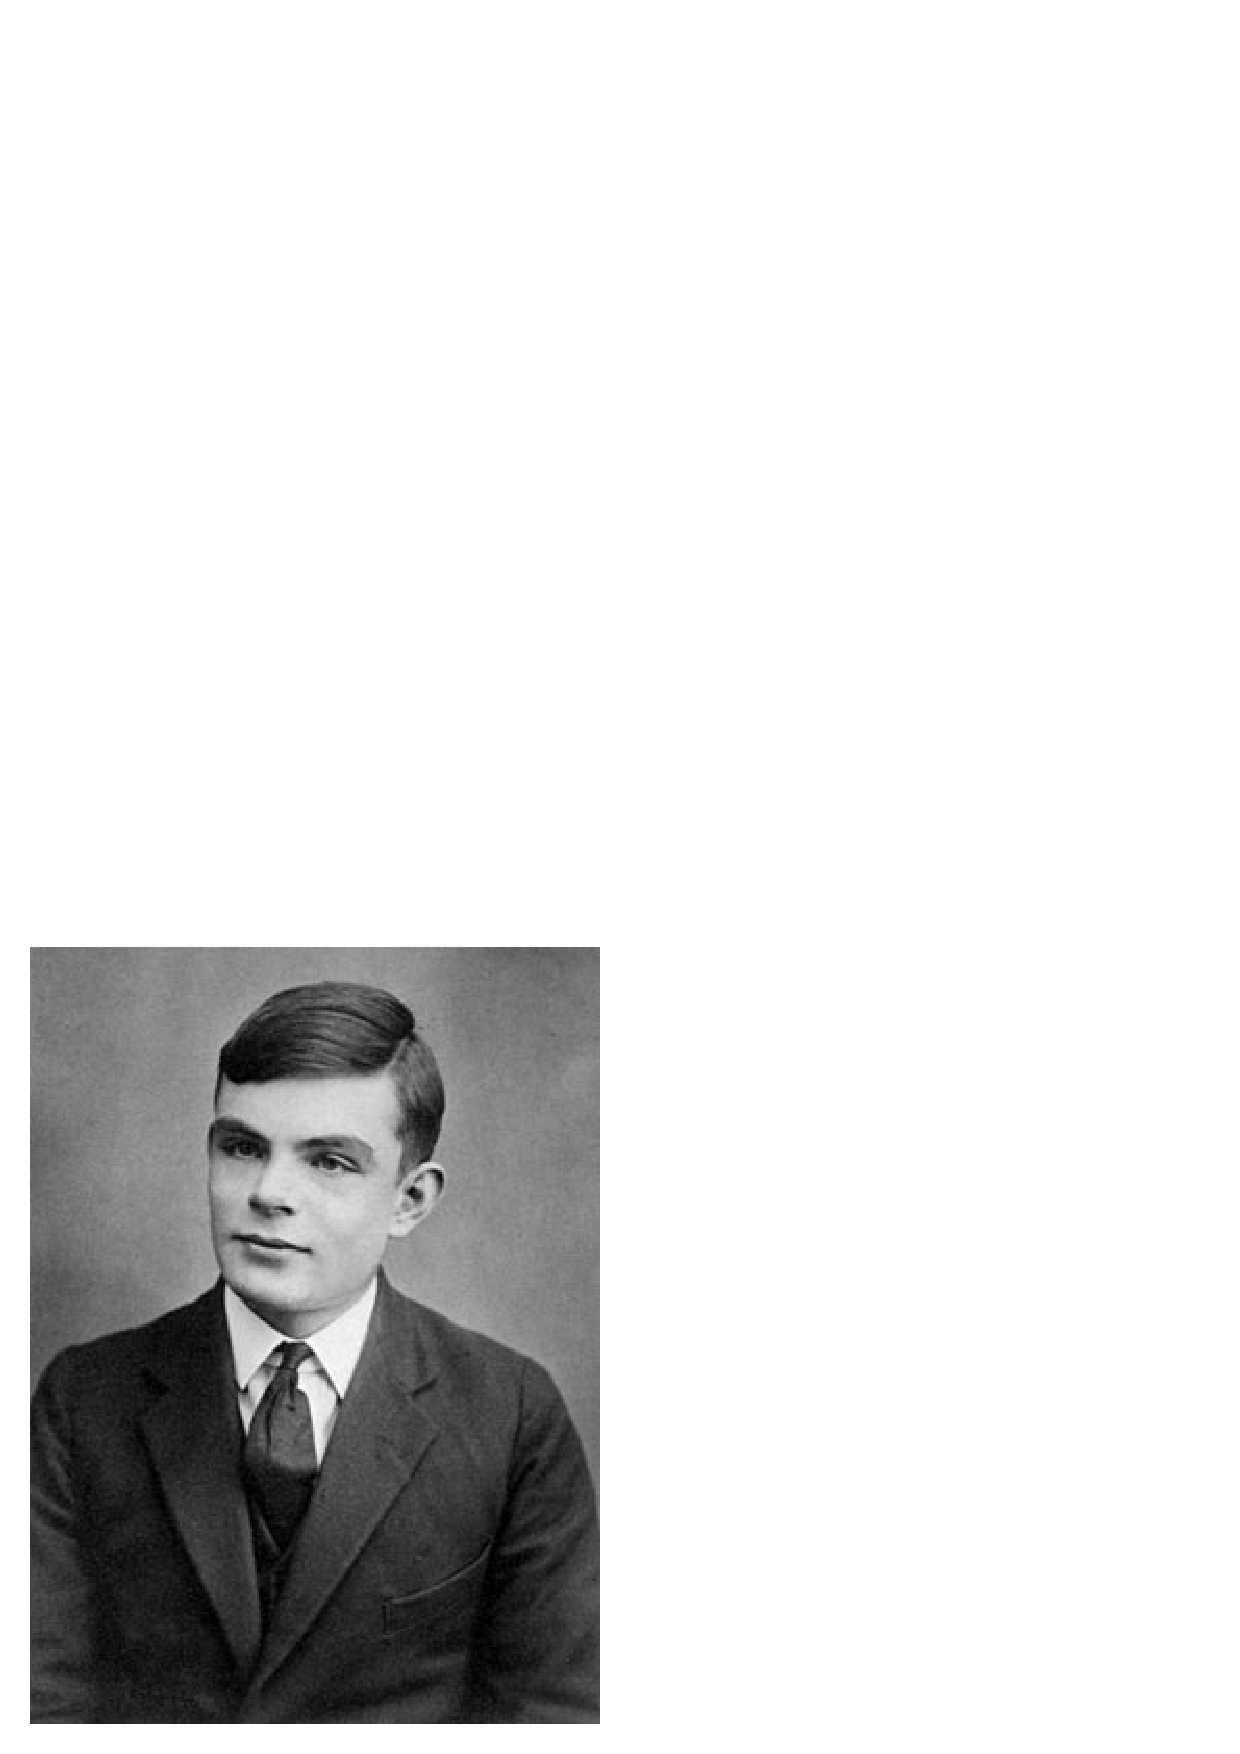
\includegraphics [scale=0.5]{ris2.png}
    \end{figure} 
 
  
 \end{block}
\end{frame}

\begin{frame}{\Large{Направления цифровизации в городе Москве}}
\begin{block}{Портал «Наш город», проект «Активный гражданин» \\ (gorod.mos.ru, ag.mos.ru)}

  \begin{figure}[htb] 
      \centering
      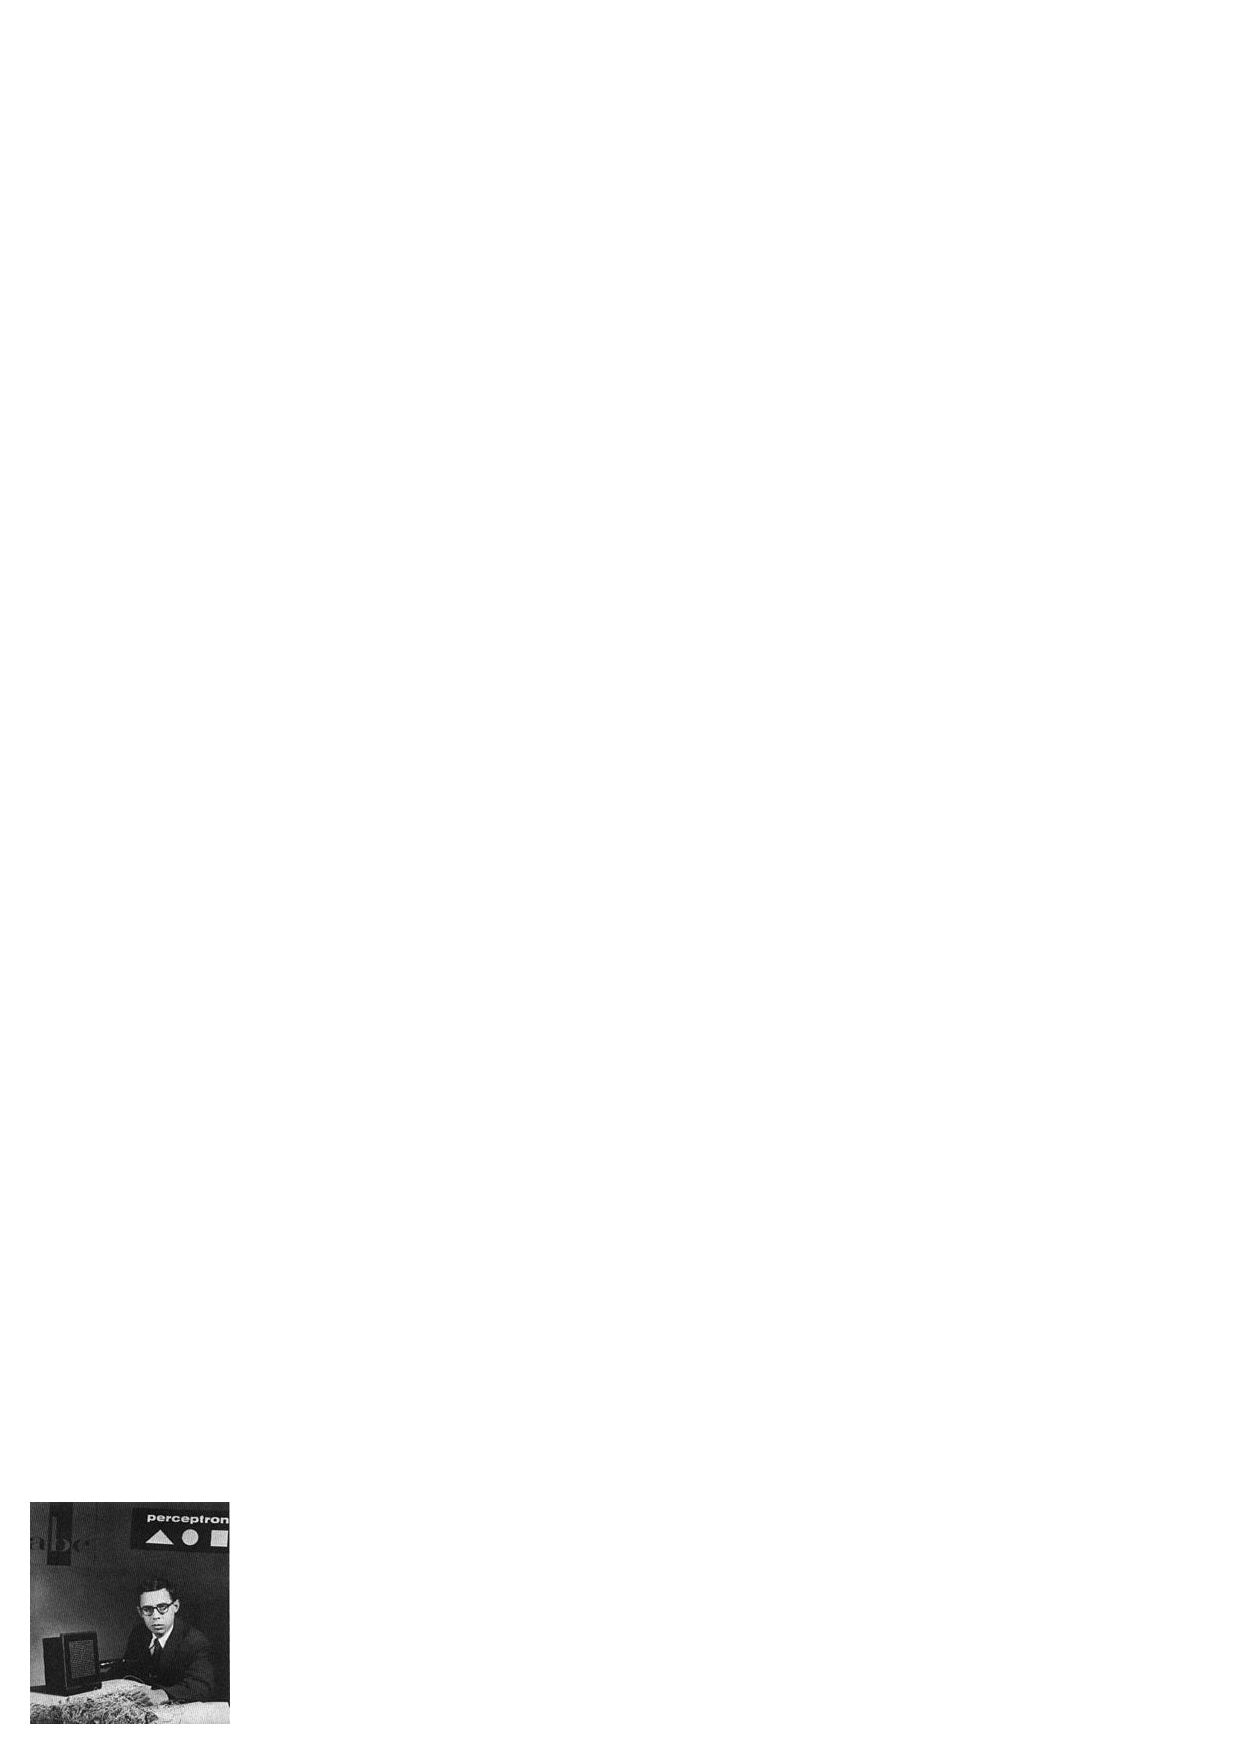
\includegraphics [scale=3.5]{ris3.png}
    \end{figure} 
 
  
 \end{block}
\end{frame}

\begin{frame}{\Large{Направления цифровизации в городе Москве}}
\begin{block}{Проект «Электронный дом» (ed.mos.ru)}

  \begin{figure}[htb] 
      \centering
      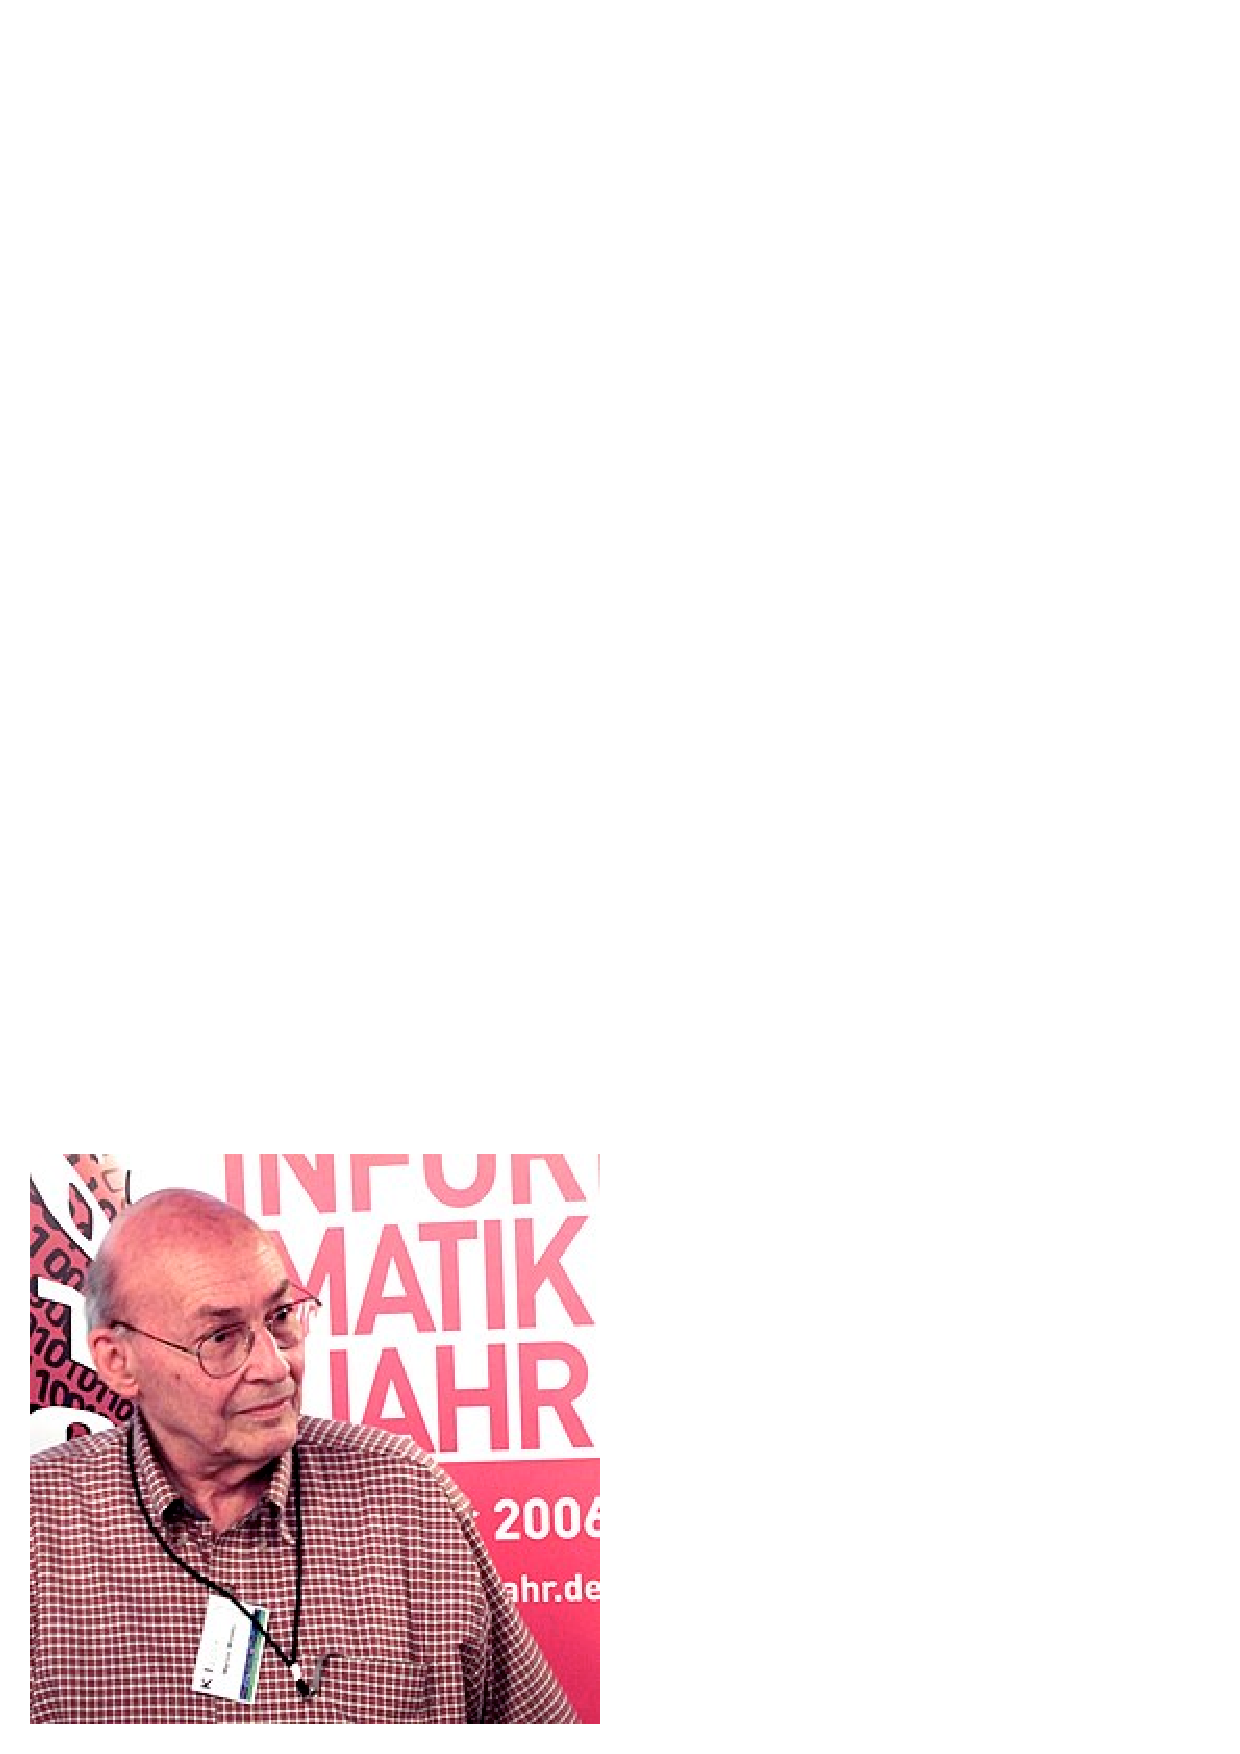
\includegraphics [scale=0.4]{ris4.png}
    \end{figure} 
 
  
 \end{block}
\end{frame}

\begin{frame}{\Large{Направления цифровизации в городе Москве}}
\begin{block}{Проект «Московская электронная школа» (school.mos.ru)}

  \begin{figure}[htb] 
      \centering
      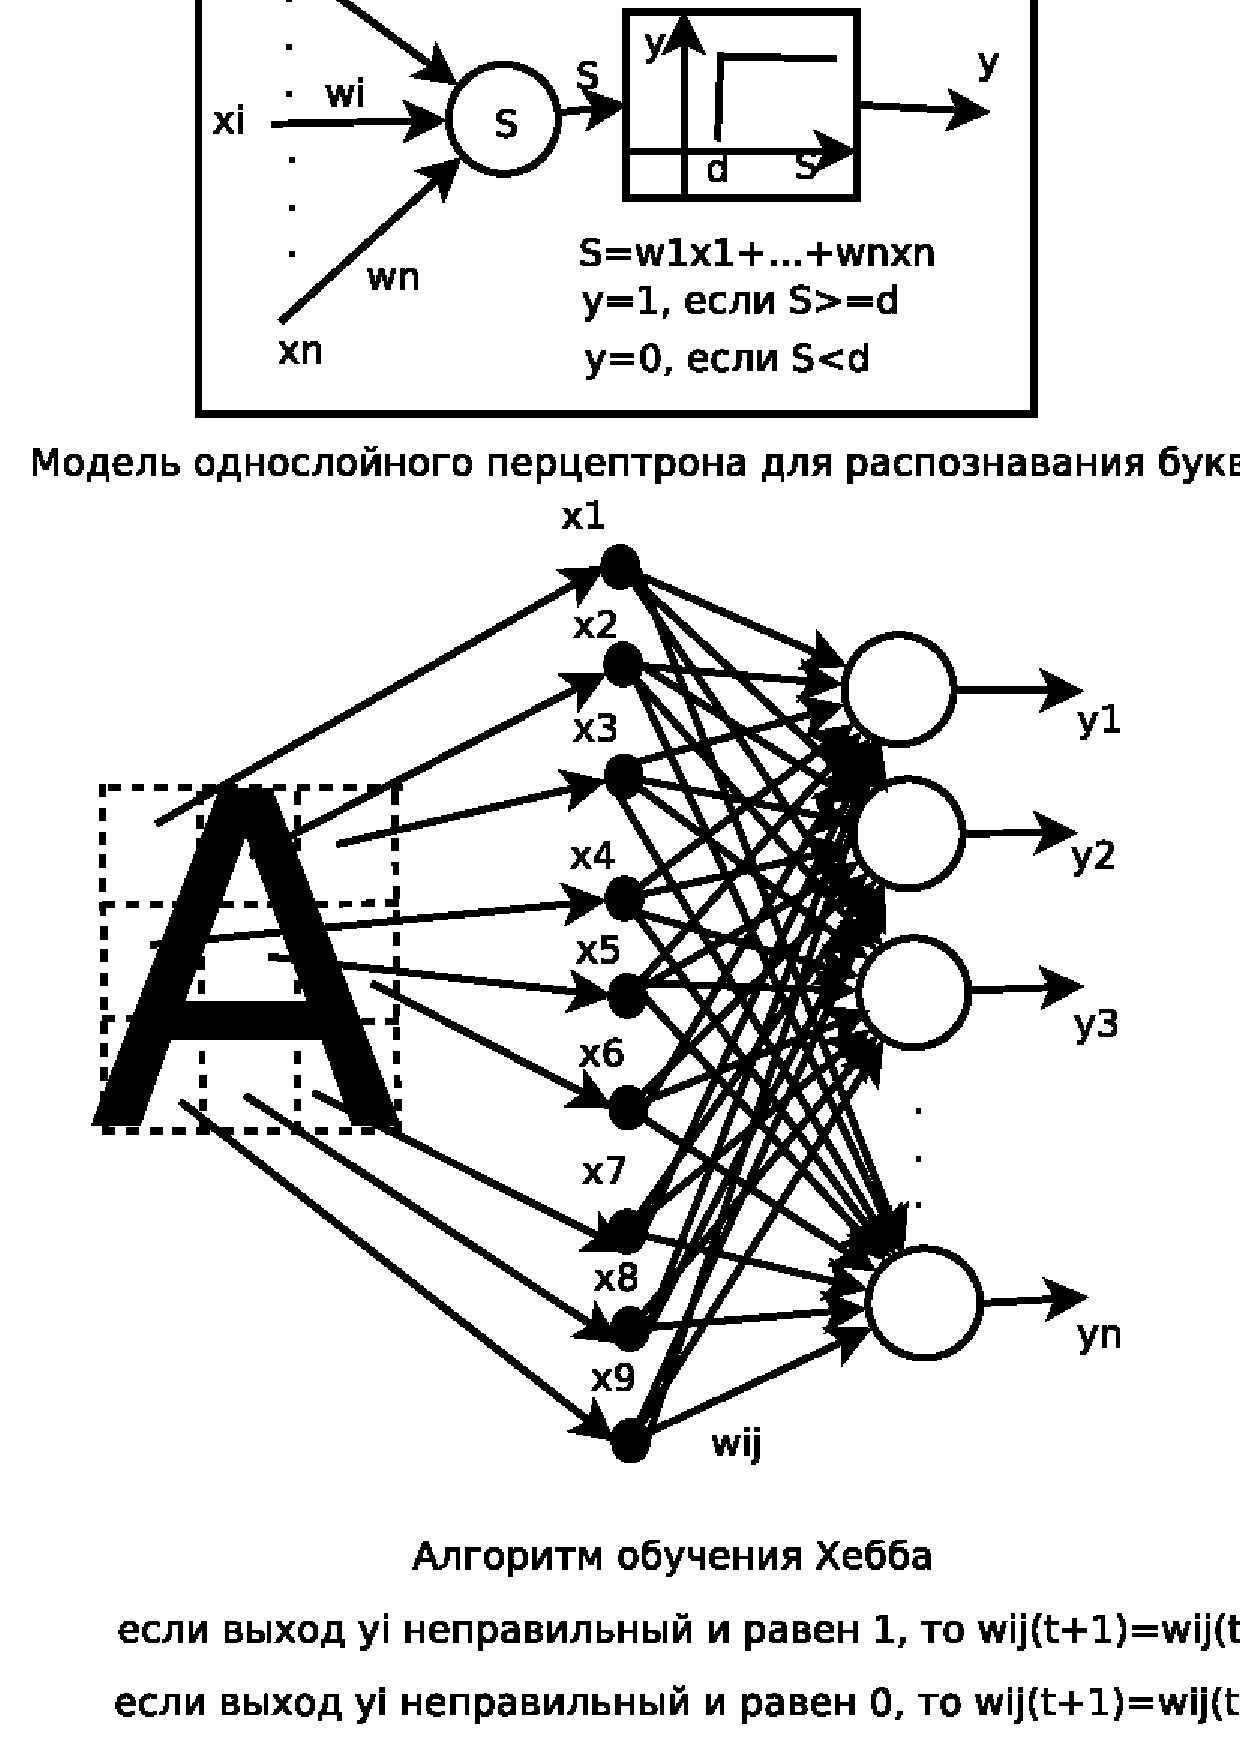
\includegraphics [scale=0.4]{ris5.png}
    \end{figure} 
 
  
 \end{block}
\end{frame}

\begin{frame}{\Large{Направления цифровизации в городе Москве}}
\begin{block}{Единая медицинская информационно-аналитическая система города Москвы (emias.info)}

  \begin{figure}[htb] 
      \centering
      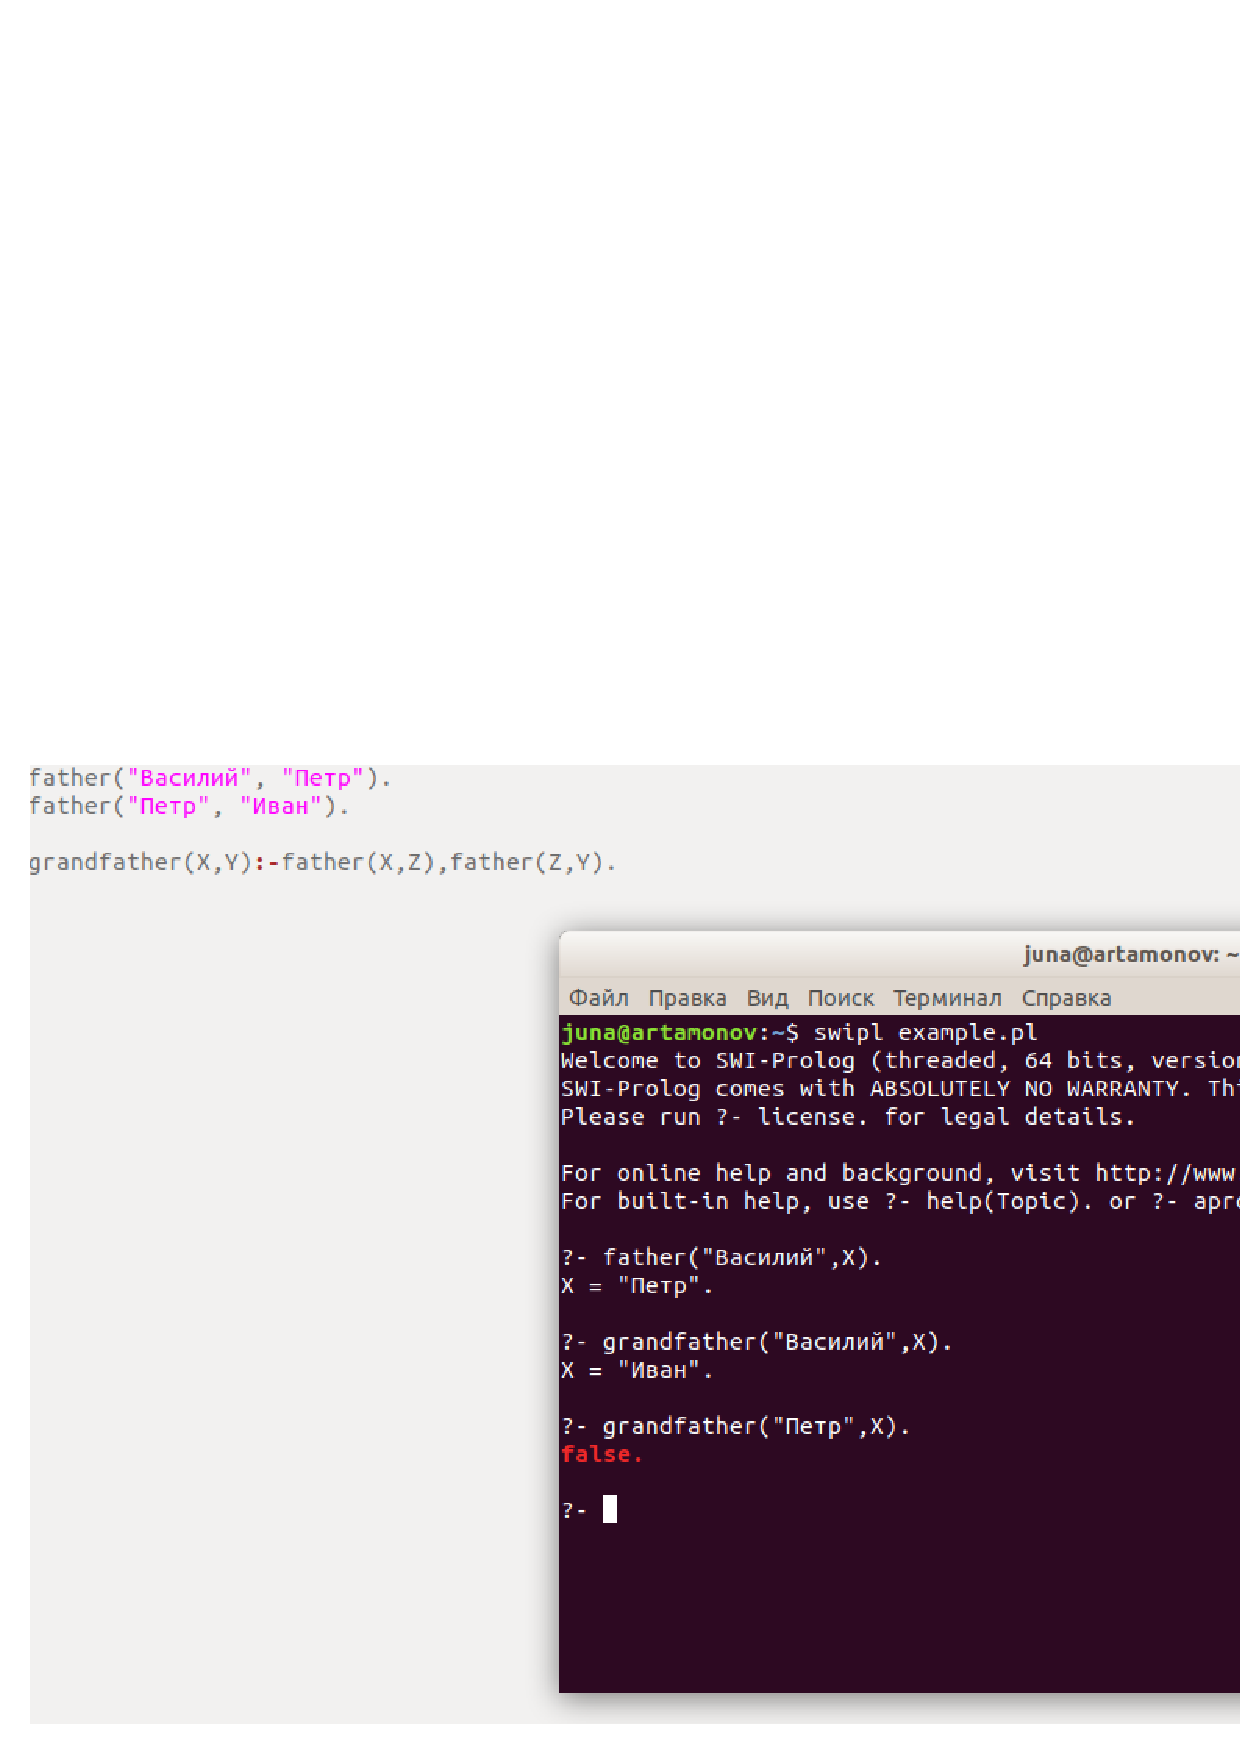
\includegraphics [scale=0.4]{ris6.png}
    \end{figure} 
 
  
 \end{block}
\end{frame}

\begin{frame}{\Large{Направления цифровизации в городе Москве}}
\begin{block}{Перечень некоторых других городских  цифровых сервисов}

  \begin{itemize}
    \item{Городская система видеонаблюдения «Единый центр  хранения и обработки данных» (echd.mos.ru)}
    \item{Автоматизированная система учета потребления ресурсов (asupr.mos.ru)}
    \item{Единый диспетчерский центр города Москвы (edc.mos.ru)}
    \item{Портал открытых данных города Москвы (https://data.mos.ru/)}
  \end{itemize}
  
 \end{block}
\end{frame}

\begin{frame}{\Large{Направления цифровизации в городе Москве}}
\begin{block}{Ситуационный зал центра управления комплекса городского хозяйства}

  \begin{figure}[htb] 
      \centering
      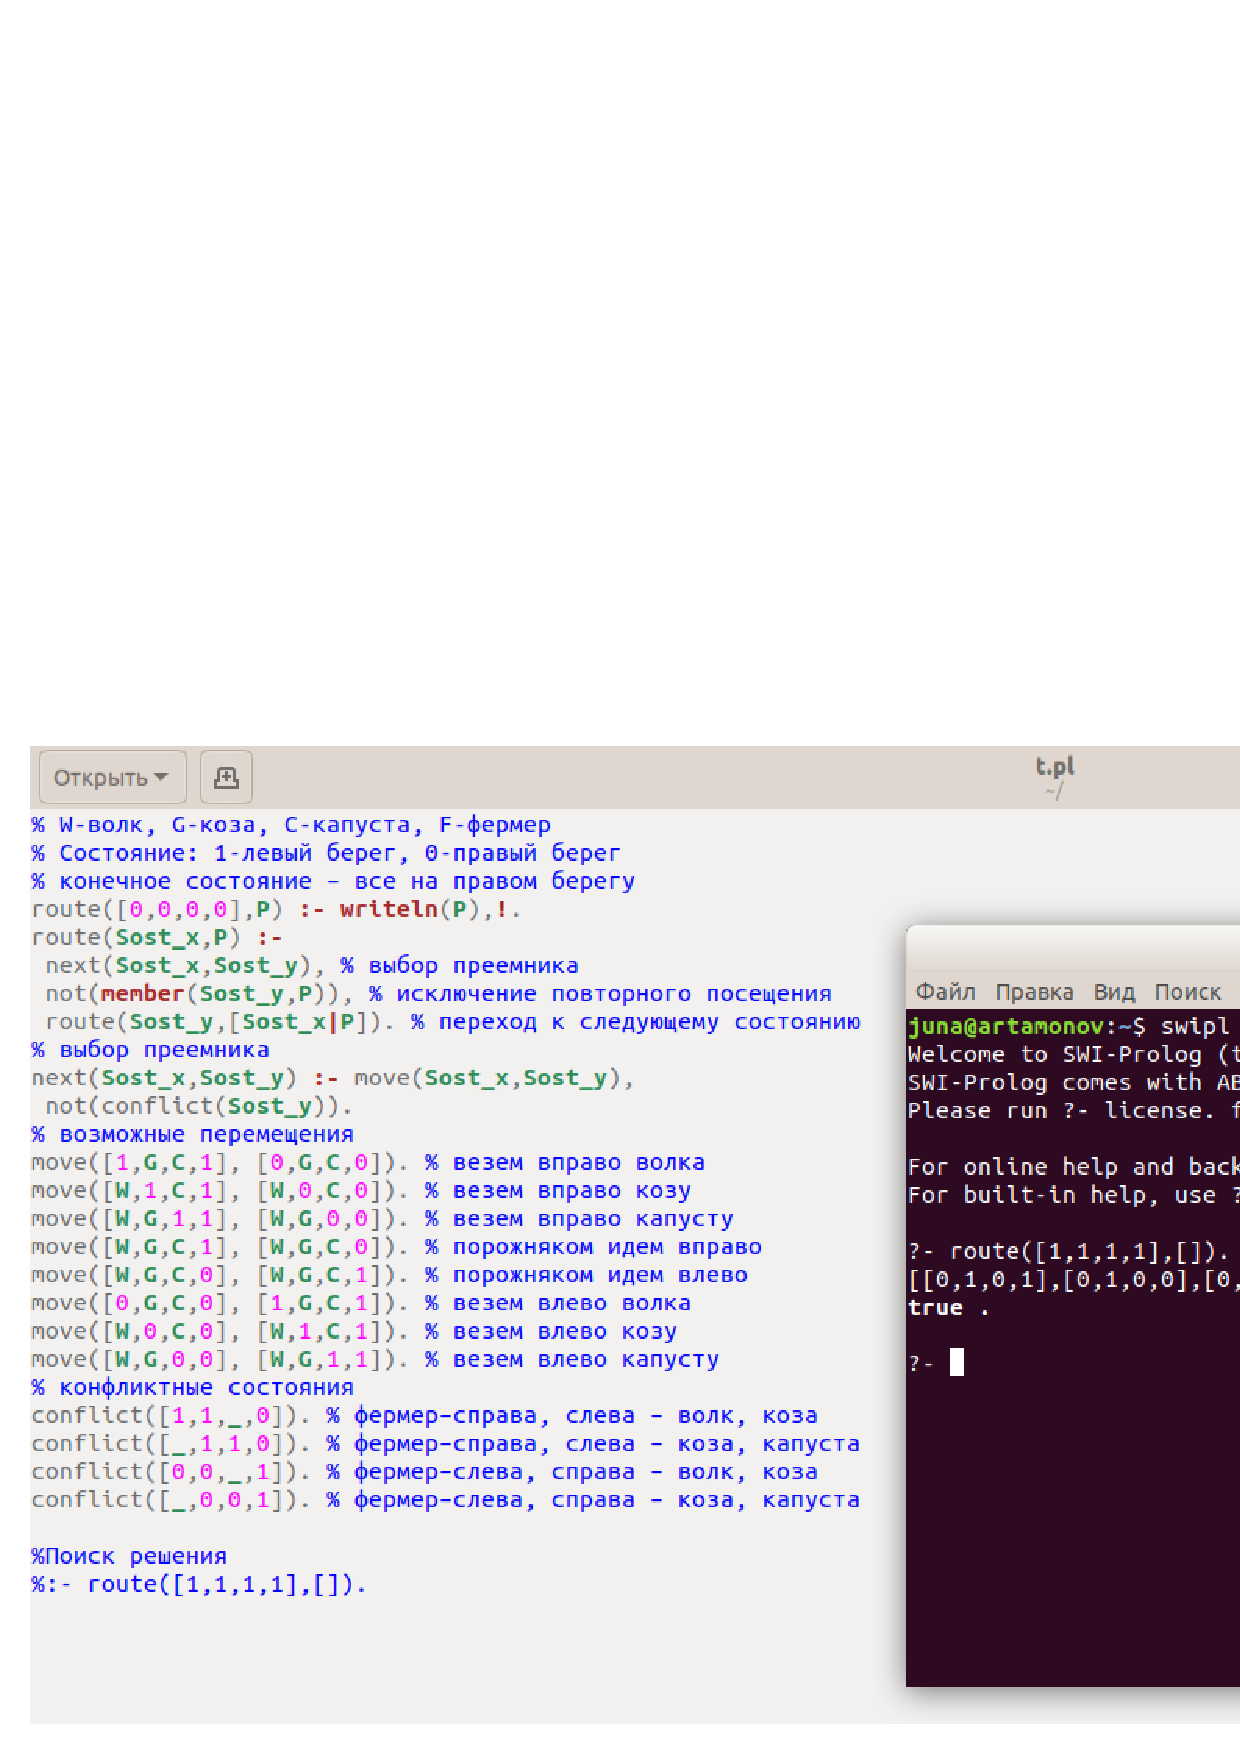
\includegraphics [scale=3.5]{ris7.png}
    \end{figure}

   Источник: материалы доклада руководителя ГБУ МАЦ
 
  
 \end{block}
\end{frame}


\begin{frame}{\Large{Направления цифровизации в городе Москве}}
\begin{block}{Главная информационная панель центра управления комплекса городского хозяйства}

  \begin{figure}[htb] 
      \centering
      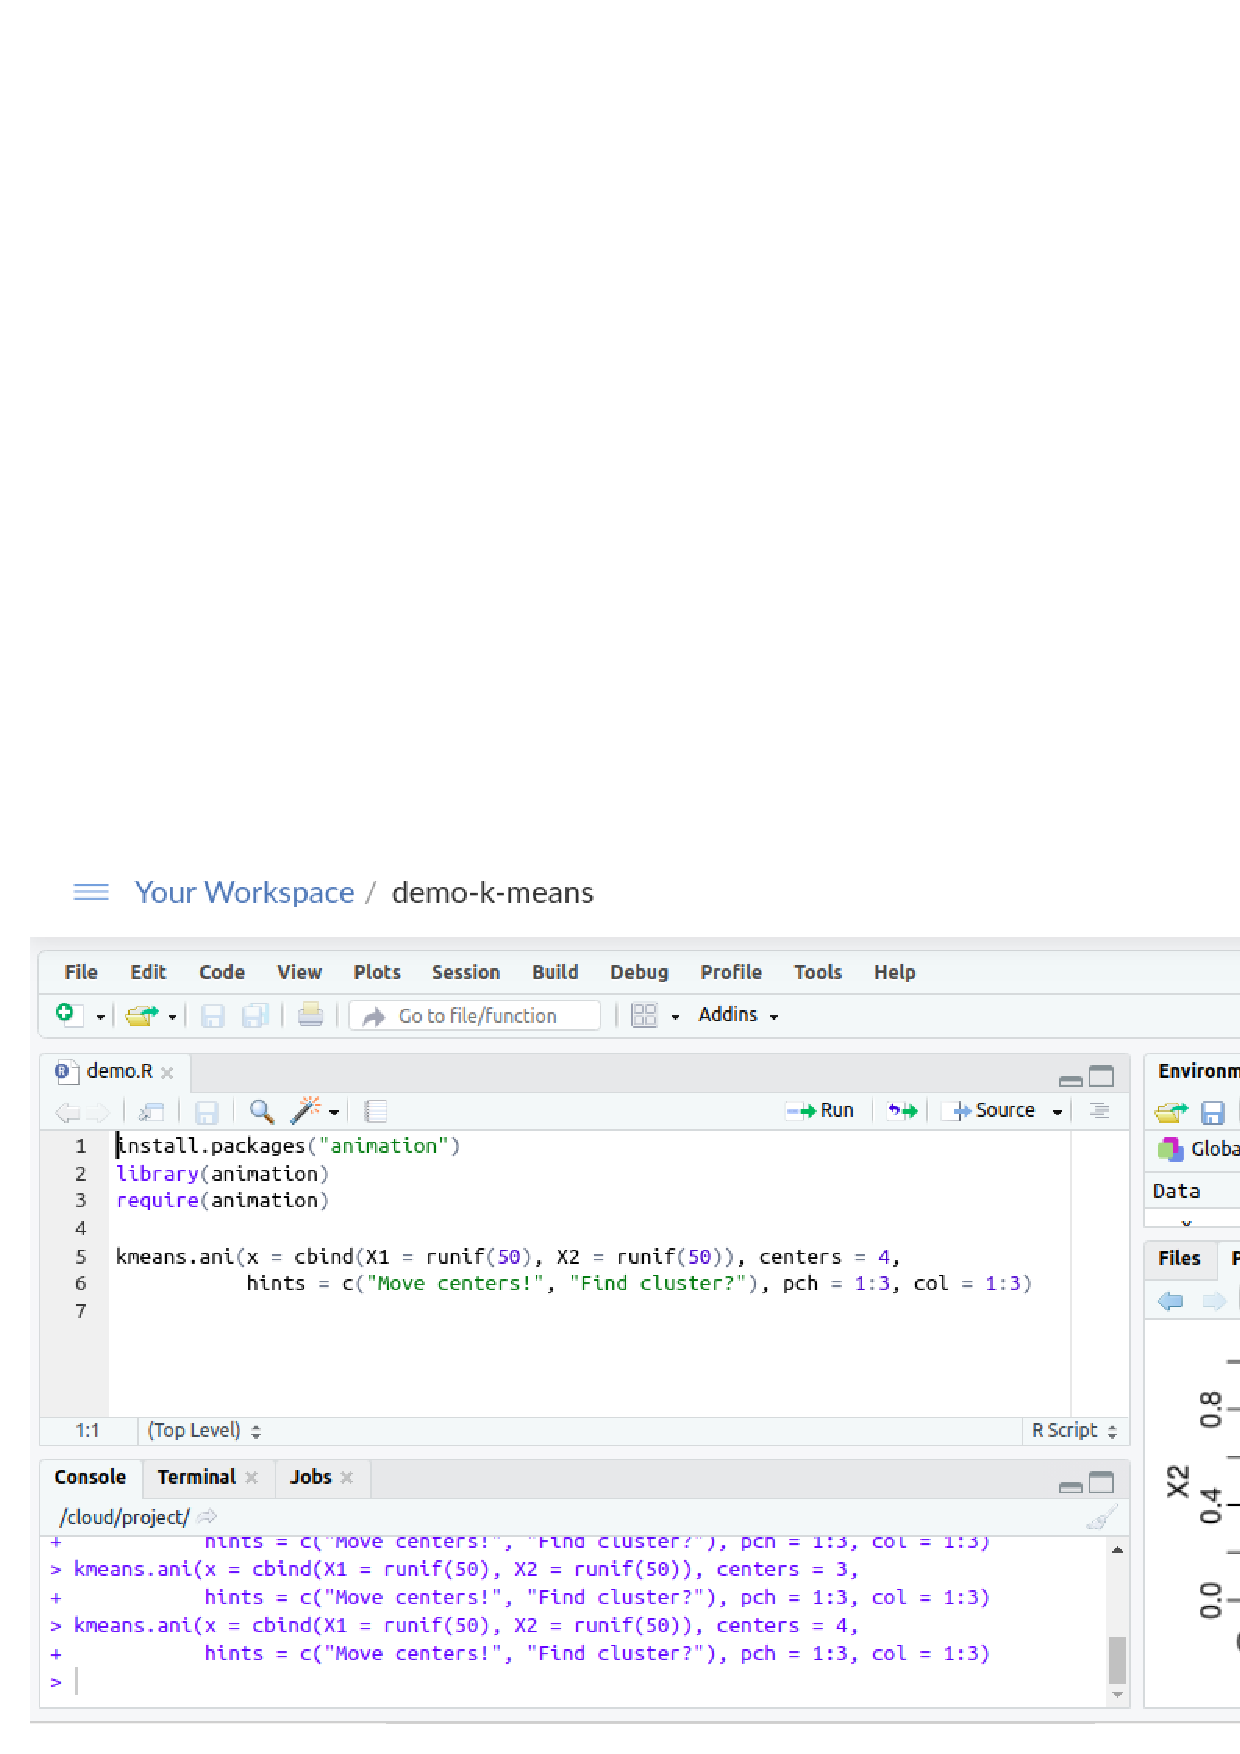
\includegraphics [scale=1.5]{ris8.png}
    \end{figure}
 
  
 \end{block}
\end{frame}


\begin{frame}{\Large{Завершение}}

  \begin{figure}[htb] 
      \centering
      \includegraphics [scale=0.9]{fin.png}
    \end{figure}


\end{frame}








\end{document}

